\chapter{Maximum common induced subgraph: the McSplit algorithm}
\label{c:mcsplit-i-undirected}

\newcommand{\BigO}[1]{\ensuremath{\operatorname{O}\left(#1\right)}}

\newcommand{\exampleG} {
    \tikz {
        \graph [nodes={draw, circle, minimum width=.55cm, inner sep=1pt}, circular placement, radius=0.95cm,
                clockwise=5] {
                    1,2,3,4,5;
            1--4; 1--5; 2--3; 2--5; 3--5;
        };
    }
}
\newcommand{\exampleH} {
    \tikz {
        \graph [nodes={draw, circle, minimum width=.55cm, inner sep=1pt}, circular placement, radius=0.95cm,
                clockwise=6, phase=60] {
                    a,b,c,d,e,f;
            a--b; a--c; a--e; b--d; b--f; c--d; c--e; c--f; d--f; e--f;
        };
    }
}

\newcommand{\LabelTables}[3] {
  {\small
    \centering
    \begin{minipage}[t]{.20\linewidth}
        Mapping

        \medskip

        #1
    \end{minipage}
    \quad
    \begin{minipage}[t]{0.31\linewidth}
        \centering
        Labelling of $\graphG$

        \begin{tabular}[t]{cc}
        \toprule
            Vertex & Label\\
        \midrule
            #2
        \bottomrule
        \end{tabular}
    \end{minipage}
    \quad
    \begin{minipage}[t]{0.31\linewidth}
        \centering
        Labelling of $\graphH$

        \begin{tabular}[t]{cc}
        \toprule
            Vertex & Label\\
        \midrule
            #3
        \bottomrule
        \end{tabular}
        \medskip
    \end{minipage}
  }
}

%%%%%%%%%%%%%%%%%%%%%%%%%%%%%%%%%%%%%%%%%%%%%%%%%%%%%%%%%%%%%%%%%%%%%%%%%%%%%%%%%%%

\section{Introduction}

To determine the similarity or difference between two graphs, we must first
find what they have in common
\citep{DBLP:journals/prl/Bunke97,DBLP:journals/prl/FernandezV01,KriegeThesis}.
The \emph{maximum common subgraph} family of problems involves finding a large
graph which is isomorphic to subgraphs of two given graphs simultaneously.
Because graphs are widely used to model real-world phenomena, maximum common
subgraph problems have arisen in molecular science (where graphs often represent
molecules)
\citep{DBLP:journals/jcamd/RaymondW02a,Ehrlich:2011,DAM2014,Grindley1993707},
and also in other domains including malware detection
\citep{DBLP:journals/compsec/ParkRS13}, source code analysis
\cite{DBLP:journals/tkde/DjokoCH97}, and computer vision
\cite{DBLP:journals/jair/CookH94}.

Maximum common subgraph problems are NP-hard, and remain challenging
computationally. Recent practical progress has been made by using constraint
programming \citep{DBLP:conf/mco/VismaraV08,DBLP:conf/cp/NdiayeS11,DBLP:conf/cp/McCreeshNPS16} and
mathematical programming \citep{DBLP:journals/dam/BahienseMPS12}, by reducing
to the maximum clique problem \citep{LeviG,DBLP:conf/cp/McCreeshNPS16}, and by
adapting subgraph isomorphism algorithms \citep{UpcomingAAAIPaper}. Some
special cases also have practical polynomial time algorithms
\citep{DBLP:conf/mfcs/DroschinskyKM16,DBLP:conf/sofsem/DroschinskyKM17}.

This chapter considers the \emph{maximum common induced subgraph} problem, in
which the objective is to find a graph with as many vertices as possible which
is an induced subgraph of each of two input graphs.  (The \emph{maximum common
partial subgraph} problem instead asks for a common non-induced subgraph with
as many \emph{edges} as possible \citep{DBLP:conf/cp/NdiayeS11}; we discuss
only the induced variant in this chapter.) We introduce
a new branch and bound algorithm which exploits special properties of the
problem to allow a much faster exploration of the search space, whilst
retaining the filtering and bounding benefits of the constraint programming
approach. We describe the algorithm for the basic maximum common subgraph
problem, and discuss how it may be adapted to handle vertex labels, edge
labels, and the requirement that the found subgraph be connected. We then
present an empirical study of the algorithm, demonstrating that it improves the
state of the art by more than an order of magnitude on the unlabelled variant
of the problem, and showing that it can handle much larger instances than
earlier constraint programming or clique approaches due to lower memory usage.

\section{The \McSplit\ Algorithm \label{sec:mcsplit}}

We initially assume that graphs are unlabelled, undirected and without loops
(\cref{sec:extensions} describes how these restrictions may be relaxed).  The
vertex and edge sets of a graph $\graphG$ are denoted $\V(\graphG)$ and
$\E(\graphG)$.  The set of vertices adjacent to vertex $v$ in graph $\graphG$
is called the \emph{neighbourhood} of $v$, denoted $\N(\graphG, v)$. We denote
by $\invN(\graphG, v)$ the \emph{inverse neighbourhood} of $v$, being the set
of the vertices not adjacent to $v$ (excluding $v$ itself). A \emph{subgraph}
of a graph $\graphG$ is a graph consisting of some of the vertices of
$\graphG$, and all of the edges between these vertices. (All subgraphs in this
chapter are induced subgraphs.) A \emph{common subgraph} of two graphs is a graph
which is (isomorphic to) a subgraph of two graphs simultaneously, and a
\emph{maximum} common subgraph is one with as many vertices as possible.

Throughout, $\graphG$ and $\graphH$ will be the two input graphs to our maximum
common subgraph problem.  The orders (number of vertices) of these graphs are
denoted $g$ and $h$ respectively.

With these definitions established, we now present \McSplit. This algorithm
finds a maximum-cardinality mapping $M^* = \{(v_1, w_1), \dots, (v_{m},
w_{m})\}$ with $|M^*| = m$ vertex pairs, where the $v_i$ are distinct vertices
from $\V(\graphG)$ and the $w_i$ are distinct vertices from $\V(\graphH)$, such
that $v_i$ and $v_j$ are adjacent in $\graphG$ if and only if $w_i$ and $w_j$
are adjacent in $\graphH$.  Given such a mapping, the subgraph of $\graphG$
induced by $\{v_1, \dots, v_{m}\}$ and the subgraph of $\graphH$ induced by
$\{w_1, \dots, w_{m}\}$ are isomorphic and correspond to a maximum common subgraph.

\paragraph{Walkthrough} Before discussing the algorithm in detail, we illustrate
the main concepts using the graphs $\graphG$ and $\graphH$ in
\cref{fig:alg1}.  These graphs have a maximum common subgraph with four
vertices; one example is the mapping $\{1a, 2f, 3d, 5b\}$ where vertex $1$ is
assigned to vertex $a$, $2$ is assigned to $f$, $3$ to $d$ and $5$ to $b$.

\begin{figure}[h!]
\centering
    \exampleG
    \qquad
    \exampleH
\caption{Example graphs $\graphG$ and $\graphH$.}
\label{fig:alg1}
\end{figure}

The algorithm builds up a mapping $M$ using a depth-first search, starting with the empty mapping
$\emptyset$ and adding a $(v_i, w_i)$ pair or choosing to leave a vertex in $\V(\graphG)$ unmatched at each level of the search tree.
Select a vertex in $\V(\graphG)$ as the first vertex to be mapped; in our
example we will arbitrarily choose vertex $1$. Each of the vertices in
$\V(\graphH)$ to which vertex $1$ may be mapped will be tried in turn, and
finally the possibility where vertex $1$ remains unmatched will be tried.

We begin by mapping vertex $1$ to vertex $a$, giving $M=\{1a\}$.  Now
label each unmatched vertex in $\V(\graphG)$ according to whether it is adjacent to vertex $1$, and
label each unmatched vertex in $\V(\graphH)$ according to whether it is adjacent to vertex $a$,
as shown in \cref{fig:alg2}.  Adjacent
vertices have label 1; non-adjacent vertices have label 0.  We can extend $M$
with a mapping $vw$, with $v \in \V(\graphG)$ and $w \in \V(\graphH)$, if and only
if $v$ and $w$ have the same label.  This property, that two vertices may be
mapped together if and only if they share a label, is the algorithm's main
invariant.

\begin{figure}[h!]
    \centering
    \subfigure[][After mapping $1$ to $a$] {
      \LabelTables{$\{1a\}$}
                  {$2$ & $0$ \\
                   $3$ & $0$ \\
                   $4$ & $1$ \\
                   $5$ & $1$ \\}
                  {$b$ & $1$ \\
                   $c$ & $1$ \\
                   $d$ & $0$ \\
                   $e$ & $1$ \\
                   $f$ & $0$ \\}
      \label{fig:alg2}
    }
    \par\bigskip
    \subfigure[][After mapping $2$ to $d$] {
      \LabelTables{$\{1a,2d\}$}
                  {$3$ & $01$ \\
                   $4$ & $10$ \\
                   $5$ & $11$ \\}
                  {$b$ & $11$ \\
                   $c$ & $11$ \\
                   $e$ & $10$ \\
                   $f$ & $01$ \\}
      \label{fig:alg3}
    }
    \par\bigskip
    \subfigure[][After mapping $3$ to $f$] {
      \LabelTables{$\{1a,2d,3f\}$}
                  {$4$ & $100$ \\
                   $5$ & $111$ \\}
                  {$b$ & $111$ \\
                   $c$ & $111$ \\
                   $e$ & $101$ \\}
      \label{fig:alg4}
    }

    \caption{Mapping $M$ and vertex labels during search on example graphs $\graphG$ and
    $\graphH$ from \cref{fig:alg1}.  Labels represent adjacencies; for example, the label
    101 on vertex $e$ in the final table signifies that $e$ is adjacent to the first
    and third mapped vertices of $\graphH$ ($a$ and $f$) but not adjacent to the second
    mapped vertex ($d$).}
    \label{figure:mcsplit-examples}
\end{figure}

Next, extend the mapping by pairing a vertex in $\graphG$ with a vertex in $\graphH$ of the
same label; we will choose to map vertex $2$ to vertex $d$, giving $M=\{1a,
2d\}$ (\cref{fig:alg3}).  Each unmapped vertex $v \in \V(\graphG)$ is labelled
with a two-character bit string, indicating its adjacency to each of
the two mapped vertices in $\V(\graphG)$ (vertices $1$ and $2$).  For example, vertex
$3$ is labelled $01$, indicating that it is not adjacent to vertex $1$ but is adjacent
to vertex $2$.  Labels are given to unmapped vertices in $\V(\graphH)$ in a similar fashion,
showing adjacency to matched vertices $a$ and $d$.  Our invariant is
maintained: we can extend $M$ by a vertex pairing if and only if the two
vertices have the same label.

The algorithm backtracks when the incumbent (the largest mapping found so far) is at least as large
as a calculated bound given $M$ and the current labelling. To demonstrate how
this bound is calculated, we consider the situation one level deeper in the
search tree shown in \cref{fig:alg4}.

Three vertex labels are used: 100,
101, and 111.  The first two of these only appear in one graph, and therefore
there is no way to add a pair of vertices with label 100 or 101 to the mapping.
The final label, 111, appears once in $\graphG$ and twice in $\graphH$, and therefore at
most one pair with this label can be added to $M$.  Thus, the upper bound on
mapping size is $|M| + 1 = 4$. The general formula for the upper bound is
\begin{multline*}
    \mathit{bound} = |M| + \sum_{l \in L} \min\big(|\{ v \in \V(\graphG) : \vtxlabel(v)=l\}|,
        |\{ v \in \V(\graphH) : \vtxlabel(v)=l \}|\big) \text{,}
\end{multline*} where $L$ is the set of labels used in both graphs.

%When we have explored the full
%search space of matchings containing $\{1a, 2d\}$, we try reassigning $2$ to
%$f$.  Since $d$ and $f$ are the only vertices to which $2$ can be matched given
%the decision to match $1$ to $a$, we lastly explore the possibility that $2$ is
%left unmatched, by giving $2$ the label $\bot$ and selecting another vertex in
%$\V(\graphG)$ to assign.

\paragraph{Label classes} We require only $\BigO{g+h}$ space per level of the
search tree to store labelling information.  This is done by storing a
\emph{label class} as a pair $\langle \setG,\setH \rangle$ for each label $l$ that is
used, where $\setG$ is the set of vertices in $\V(\graphG)$ labelled $l$, and $\setH$ is the
set of vertices in $\V(\graphH)$ labelled $l$. Since there are $g + h$ vertices in the two graphs, at most
$g + h$ label classes can exist at once, and there are at most $g + h$ vertices
in the union of all of the $\setG$ and $\setH$ sets. Furthermore, we do not actually
need to store the bits making up a label---we care only that like-labelled
vertices are kept together, and the label itself is not used. Nor do we need to
store any label class which is present only in one graph but not the other (or
which is not present at all).

Together, these facts allow us to store all the
necessary information in three arrays.  The first 
stores a permutation of $\V(\graphG)$ in which like-labelled vertices appear
consecutively.  The second array, similarly, stores a permutation
of $\V(\graphH)$ with like-labelled vertices together.  We call these
the \emph{G-array} and \emph{H-array} respectively. The third array,
which we call the \emph{LC-array},
contains a record for each label class $\langle \setG,\setH \rangle$.  Each
record contains start and end pointers to the portion of the
G-array that contains $\setG$, and start and end pointers to the portion
of the H-array that contains $\setH$.
This representation has
similarities to data structures used in partition backtracking for graph isomorphism
\citep{DBLP:conf/wea/Lopez-PresaA09,DBLP:journals/jsc/McKayP14} and the \citet{DBLP:journals/cacm/BronK73}
clique enumeration algorithm.  TODO: say more about similarities and differences

\Cref{fig:data-structure} illustrates this data structure using our running example.
The first subfigure shows the initial label classes when no vertex assignments have
been made; the second and third subfigures correspond to the first two steps in \Cref{figure:mcsplit-examples}.
Each subfigure shows graphs $\graphG$ and $\graphH$ with vertices colour-coded according
to their label class.  The three arrays of our data structure are shown on the right of each subfigure,
with the LC-array below the G-array and H-array.  The grey numbers below the G-array and H-array
are the array indices; these are not stored explicitly.

\begin{figure}[h!]
\newcommand{\ColouredGraphG}[5] {
    \begin{tikzpicture}[scale=0.35]
        \tikz {
            \graph [nodes={draw, circle, minimum width=.45cm, inner sep=1pt}, circular placement, radius=0.75cm,
                    clockwise=5] {
                        1[fill=#1],2[fill=#2],3[fill=#3],4[fill=#4],5[fill=#5];
                1--4; 1--5; 2--3; 2--5; 3--5;
            };
        }
    \end{tikzpicture}   
}
\newcommand{\ColouredGraphH}[6] {
    \begin{tikzpicture}[scale=0.35]
        \tikz {
            \graph [nodes={draw, circle, minimum width=.45cm, inner sep=1pt}, circular placement, radius=0.75cm,
                    clockwise=6, phase=60] {
                        a[fill=#1],b[fill=#2],c[fill=#3],d[fill=#4],e[fill=#5],f[fill=#6];
                a--b; a--c; a--e; b--d; b--f; c--d; c--e; c--f; d--f; e--f;
            };
        }
    \end{tikzpicture}   
}
\newcommand{\DataStructureGridsG}[5] {
    \fill[#1] (1,0) rectangle ++ (1,1); 
    \fill[#2] (2,0) rectangle ++ (1,1); 
    \fill[#3] (3,0) rectangle ++ (1,1); 
    \fill[#4] (4,0) rectangle ++ (1,1); 
    \fill[#5] (5,0) rectangle ++ (1,1); 
    \foreach \x in {1,...,5} {\node at (\x+.5,-0.4) {{\color{black!60}\footnotesize{\pgfmathprintnumber{\x}}}}; }
    \draw[step=1cm,black,thin] (1,0) grid (6,1);
}

\newcommand{\DataStructureGridsH}[6] {
    \fill[#1] (7,0) rectangle ++ (1,1); 
    \fill[#2] (8,0) rectangle ++ (1,1); 
    \fill[#3] (9,0) rectangle ++ (1,1); 
    \fill[#4] (10,0) rectangle ++ (1,1); 
    \fill[#5] (11,0) rectangle ++ (1,1); 
    \fill[#6] (12,0) rectangle ++ (1,1); 
    \foreach \x in {1,...,6} {\node at (\x+6.5,-0.4) {{\color{black!60}\footnotesize{\pgfmathprintnumber{\x}}}}; }
    \draw[step=1cm,black,thin] (7,0) grid (13,1);
}

\centering
    \subfigure[][Before mapping any vertices] {
        \ColouredGraphG{uofglawn!60}{uofglawn!60}{uofglawn!60}{uofglawn!60}{uofglawn!60}
        \quad
        \ColouredGraphH{uofglawn!60}{uofglawn!60}{uofglawn!60}{uofglawn!60}{uofglawn!60}{uofglawn!60}
        \qquad
        \qquad
        \begin{tikzpicture}[scale=0.5]
            \DataStructureGridsG{uofglawn!60}{uofglawn!60}{uofglawn!60}{uofglawn!60}{uofglawn!60}
            \DataStructureGridsH{uofglawn!60}{uofglawn!60}{uofglawn!60}{uofglawn!60}{uofglawn!60}{uofglawn!60}

            \foreach \x/\v in {1/1,2/2,3/3,4/4,5/5} {\node at (\x+.5,0.5) {\pgfmathprintnumber{\v}}; }
            \foreach \x/\v in {1/a,2/b,3/c,4/d,5/e,6/f} {\node at (\x+6.5,0.5) {\v}; }

            \draw[fill=uofglawn!60] (5.5,-3) rectangle ++ (3,1); 
            \draw (5.3,-3.2) rectangle ++ (3.4,1.4); 
            \node at (7,-2.5) {$1,5,1,6$};

            \draw [-stealth](6,-2) -- (3.5,-1.2);
            \draw [-stealth](8,-2) -- (10,-1.2);
            \draw [decorate, decoration = {calligraphic brace, mirror, amplitude=5pt}] (1,-.8) -- ++ (5,0);
            \draw [decorate, decoration = {calligraphic brace, mirror, amplitude=5pt}] (7,-.8) -- ++ (6,0);
        \end{tikzpicture}   
        \label{subfig:data-structure-a}
    }
    \par\bigskip
    \subfigure[][After mapping $1$ to $a$] {
        \ColouredGraphG{none}{uofgsandstone!60}{uofgsandstone!60}{uofglavendar!60}{uofglavendar!60}
        \quad
        \ColouredGraphH{none}{uofglavendar!60}{uofglavendar!60}{uofgsandstone!60}{uofglavendar!60}{uofgsandstone!60}
        \qquad
        \qquad
        \begin{tikzpicture}[scale=0.5]
            \DataStructureGridsG{uofgsandstone!60}{uofgsandstone!60}{uofglavendar!60}{uofglavendar!60}{white}
            \DataStructureGridsH{uofgsandstone!60}{uofgsandstone!60}{uofglavendar!60}{uofglavendar!60}{uofglavendar!60}{white}

            \foreach \x/\v in {1/2,2/3,3/4,4/5,5/1} {\node at (\x+.5,0.5) {\pgfmathprintnumber{\v}}; }
            \foreach \x/\v in {1/d,2/f,3/b,4/c,5/e,6/a} {\node at (\x+6.5,0.5) {\v}; }

            \draw[fill=uofgsandstone!60] (5.5-2.001,-3) rectangle ++ (3,1); 
            \node at (7-2.001,-2.5) {$1,2,1,2$};

            \draw[fill=uofglavendar!60] (5.5+2.001,-3) rectangle ++ (3,1); 
            \node at (7+2.001,-2.5) {$3,4,3,5$};
            \draw (5.3-2.001,-3.2) rectangle ++ (7.4,1.4); 

            \draw [-stealth](6-2.001,-2) -- (2,-1.2);
            \draw [-stealth](8-2.001,-2) -- (8,-1.2);
            \draw [decorate, decoration = {calligraphic brace, mirror, amplitude=5pt}] (1,-.8) -- ++ (2,0);
            \draw [decorate, decoration = {calligraphic brace, mirror, amplitude=5pt}] (7,-.8) -- ++ (2,0);

            \draw [-stealth](6+2.001,-2) -- (4,-1.2);
            \draw [-stealth](8+2.001,-2) -- (10.5,-1.2);
            \draw [decorate, decoration = {calligraphic brace, mirror, amplitude=5pt}] (3,-.8) -- ++ (2,0);
            \draw [decorate, decoration = {calligraphic brace, mirror, amplitude=5pt}] (9,-.8) -- ++ (3,0);
        \end{tikzpicture}   
        \label{subfig:data-structure-b}
    }
    \par\bigskip
    \subfigure[][After mapping $2$ to $d$] {
        \ColouredGraphG{none}{none}{uofgpumpkin!60}{uofgthistle!60}{uofgpillarbox!60}
        \quad
        \ColouredGraphH{none}{uofgpillarbox!60}{uofgpillarbox!60}{none}{uofgthistle!60}{uofgpumpkin!60}
        \qquad
        \qquad
        \begin{tikzpicture}[scale=0.5]
            \DataStructureGridsG{uofgpumpkin!60}{white}{uofgthistle!60}{uofgpillarbox!60}{white}
            \DataStructureGridsH{uofgpumpkin!60}{white}{uofgthistle!60}{uofgpillarbox!60}{uofgpillarbox!60}{white}

            \foreach \x/\v in {1/3,2/2,3/4,4/5,5/1} {\node at (\x+.5,0.5) {\pgfmathprintnumber{\v}}; }
            \foreach \x/\v in {1/f,2/d,3/e,4/b,5/c,6/a} {\node at (\x+6.5,0.5) {\v}; }

            \draw[fill=uofgpumpkin!60] (5.5-4.001,-3) rectangle ++ (3,1); 
            \node at (7-4.001,-2.5) {$1,1,1,1$};

            \draw[fill=uofgthistle!60] (5.5,-3) rectangle ++ (3,1); 
            \node at (7,-2.5) {$3,3,3,3$};

            \draw[fill=uofgpillarbox!60] (5.5+4.001,-3) rectangle ++ (3,1); 
            \node at (7+4.001,-2.5) {$4,4,4,5$};

            \draw (5.3-4.001,-3.2) rectangle ++ (11.5,1.4); 

            \draw [-stealth](6-4.001,-2) -- (1.5,-1.2);
            \draw [-stealth](8-4.001,-2) -- (7.5,-1.2);
            \draw [decorate, decoration = {calligraphic brace, mirror, amplitude=5pt}] (1,-.8) -- ++ (1,0);
            \draw [decorate, decoration = {calligraphic brace, mirror, amplitude=5pt}] (7,-.8) -- ++ (1,0);

            \draw [-stealth](6,-2) -- (3.5,-1.2);
            \draw [-stealth](8,-2) -- (9.5,-1.2);
            \draw [decorate, decoration = {calligraphic brace, mirror, amplitude=5pt}] (3,-.8) -- ++ (1,0);
            \draw [decorate, decoration = {calligraphic brace, mirror, amplitude=5pt}] (9,-.8) -- ++ (1,0);

            \draw [-stealth](6+4.001,-2) -- (4.5,-1.2);
            \draw [-stealth](8+4.001,-2) -- (11,-1.2);
            \draw [decorate, decoration = {calligraphic brace, mirror, amplitude=5pt}] (4,-.8) -- ++ (1,0);
            \draw [decorate, decoration = {calligraphic brace, mirror, amplitude=5pt}] (10,-.8) -- ++ (2,0);
        \end{tikzpicture}   
        \label{subfig:data-structure-c}
    }
\caption{An illustration of McSplit's data structure for representing label classes. In each subfigure,
graphs $\graphG$ and $\graphH$ are shown on the left and our data structure for representing label classes
is shown on the right. Vertices in the same label class are shown in the same colour; white vertices
do not belong to any label class.}
\label{fig:data-structure}
\end{figure}

When the algorithm begins, all vertices in the two graphs are in a single label class, as
shown in \Cref{subfig:data-structure-a}.  The LC-array has a single element, $1,5,1,6$; this indicates
that the label class contains the vertices in positions 1 to 5 of the G-array and positions 1 to 6
of the H-array.

The label classes after mapping vertex 1 to vertex $a$ are shown in \Cref{subfig:data-structure-b}.
The grey label class shows vertices that are not adjacent to vertex 1 or vertex $a$; the purple
label class shows adjacent vertices.  The LC-array contains an element for each of these label
classes, with pointers into the G-array and H-array.

The situation after the additional mapping of 2 to $d$ is shown in \Cref{subfig:data-structure-c}.
There are now three label classes, and three corresponding members of the LC-array.

We will describe how the data structure is updated after presenting the McSplit algorithm in detail.

\begin{algorithm}[h!]
\DontPrintSemicolon
\nl $\FuncSty{Search}(\AlgVar{future},M)$ \;
\nl \Begin{
%\nl \lIf {$\AlgVar{future} = \emptyset$ \bf{and} $|M| > |\AlgVar{incumbent}|$}
\nl \lIf {$|M| > |\AlgVar{incumbent}|$}{$\AlgVar{incumbent} \gets M$} \label{StoreIncumbent}
%\nl \lIf {$\AlgVar{future} = \emptyset$}{return}
\medskip
\nl $\AlgVar{bound} \gets |M|  + \sum_{\langle \setG,\setH \rangle \in \AlgVar{future}} \min(|\setG|,|\setH|)$ \label{CalcBound} \;
\nl \lIf {$\AlgVar{bound} \leq |\AlgVar{incumbent}|$}{\KwSty{return}} \label{PruneSearch}
\medskip
\nl $\langle \setG,\setH \rangle \gets \FuncSty{SelectLabelClass}(\AlgVar{future})$ \label{SelectClass} \;
\nl $v \gets \FuncSty{SelectVertex}(\setG)$ \label{SelectVertex} \;
\nl \For {$w \in \setH$ \label{WLoop}} {
\nl    $\AlgVar{future'} \gets \emptyset$ \label{NewFuture} \;
\nl    \For {$\langle \setG',\setH'\rangle \in future$ \label{InnerLoop}}{
\nl        $\setG'' \gets \setG' \cap \N(\graphG, v) \setminus \{v\}$ \label{NewPWithEdge} \;
\nl        $\setH'' \gets \setH' \cap \N(\graphH, w) \setminus \{w\}$ \;
\nl        \If {$\setG'' \neq \emptyset$ \bf{and} $\setH'' \neq \emptyset$\label{IfNonEmpty}}{
\nl            $\AlgVar{future'} \gets \AlgVar{future'} \cup \{\langle \setG'' , \setH'' \rangle\}$ \label{AddToFutureWithEdge}}
\nl        $\setG'' \gets \setG' \cap \invN(\graphG, v) \setminus \{v\}$ \label{NewPWithoutEdge}  \;
\nl        $\setH'' \gets \setH' \cap \invN(\graphH, w) \setminus \{w\}$ \;
\nl        \If {$\setG'' \neq \emptyset$ \bf{and} $\setH'' \neq \emptyset$\label{IfNonEmpty2}}{
\nl            $\AlgVar{future'} \gets \AlgVar{future'} \cup \{\langle \setG'' , \setH'' \rangle\}$} \label{InnerLoopEnd}
       }
\nl   $\FuncSty{Search}(\AlgVar{future'},M\cup \{(v,w)\})$ \label{ExpandWithV} \;
  }
\nl $\setG' \gets \setG \setminus \{v\}$ \label{RemoveV} \;
\nl $\AlgVar{future} \gets \AlgVar{future} \setminus \{\langle \setG,\setH \rangle\}$\;
\nl \lIf {$\setG' \neq \emptyset$} {$\AlgVar{future} \gets \AlgVar{future} \cup \{\langle \setG',\setH \rangle \}$}
\nl $\FuncSty{Search}(\AlgVar{future},M)$ \label{ExpandWithoutV} \;
}
\;
\nl $\FuncSty{McSplit}(\graphG,\graphH)$ \label{McSplitFun} \;
\nl \Begin{
    \nl $\KwSty{global}~\AlgVar{incumbent} \gets \emptyset$ \;
\nl $\FuncSty{Search}(\{\langle V(\graphG),V(\graphH) \rangle \},\emptyset)$ \label{FirstExpandCall} \;
\nl $\KwSty{return}$~$\AlgVar{incumbent}$ \;
}
\caption{McSplit: a branch-and-bound algorithm to find a maximum common induced subgraph of two graphs.}
\label{McSplitAlg}
\end{algorithm}

\paragraph{\cref{McSplitAlg} in detail} We start our search at the function
$\FuncSty{McSplit}$ (\lineref{McSplitFun}),
with graphs $\graphG$ and $\graphH$ as inputs.  This function returns a mapping of
maximum cardinality.  In \lineref{FirstExpandCall} the initial call is made to
$\FuncSty{Search}$; at this point we have a single label-class containing all
vertices, and the mapping $M$ is empty.

The recursive procedure,
$\FuncSty{Search}$, has two parameters.  The parameter $\AlgVar{future}$ is a
list of label classes, each represented as a $\langle \setG, \setH \rangle$ pair as
described above.  The parameter $M$ is the current mapping of vertices.  On
each call to $\FuncSty{Search}$, the invariant holds that a $(v,w)$ pair may be
added to $M$ if and only if $v$ and $w$ belong to the same label class in
$\AlgVar{future}$.

\Lineref{StoreIncumbent} stores the current mapping $M$ if it is large enough
to unseat the incumbent.  \Linerangeref{CalcBound}{PruneSearch} prune the
search when a calculated upper bound is not larger than the incumbent.

The remainder of the procedure performs the search.  A label class
$\langle \setG, \setH \rangle$ is selected from $\AlgVar{future}$
using some heuristic
(\lineref{SelectClass}); from this label class, a vertex $v$ is selected
from $\setG$ (\lineref{SelectVertex}). We now iterate over all
vertices $w$ in $\setH$, exploring the consequences of adding $(v,w)$ to $M$
(\linerangeref{WLoop}{ExpandWithV}).  A new set of label-classes,
$\AlgVar{future'}$,
is created (\lineref{NewFuture}); this will be the labelling that results
from adding $(v,w)$ to our mapping.  Every label-class in $\AlgVar{future}$ can
now be split (\linerangeref{InnerLoop}{InnerLoopEnd}) into two new classes. The
first of these classes (\linerangeref{NewPWithEdge}{AddToFutureWithEdge})
contains vertices in $\setG$ adjacent to $v$ and vertices in $\setH$ adjacent to $w$.
This is added to $\AlgVar{future'}$ if both sets contain at least one vertex.
This is then repeated symmetrically for non-adjacency
(\linerangeref{NewPWithoutEdge}{InnerLoopEnd}). A recursive call is made
(\lineref{ExpandWithV}), on return from which we remove the mapping $(v,w)$.
Having explored all possible mappings of $v$ with vertices in $\setH$ we now
consider what happens if $v$ is not matched
(\linerangeref{RemoveV}{ExpandWithoutV}).

\paragraph{Updating the data structure}
We now return to the data structure illustrated in \Cref{fig:data-structure}, and describe
our implementation of \linerangeref{InnerLoop}{InnerLoopEnd} of the algorithm.
We use a simple $\BigO{g+h}$-time procedure to create $\AlgVar{future'}$.
First, $v$ is removed from its label class by swapping it with the rightmost
element of its label class in the G-array and decrementing the corresponding
pointer in the LC-array. Vertex $w$ is removed in a similar manner.
Next, the following procedure, corresponding to lines \linerangeref{NewPWithEdge}{InnerLoopEnd}
is carried out for each label class $\langle \setG,\setH \rangle$.  The sub-array
of the G-array corresponding to $\setG$ is partitioned such that all vertices adjacent to $v$ are moved to
the rightmost part of the sub-array. Similarly, the sub-array of the H-array corresponding to $\setH$
is partitioned in order to move all vertices adjacent to $w$ to the right.
If, after this partitioning procedure, the right-hand portion of both of these subarrays
has nonzero length, we create a new LC-array element pointing to these right-hand portions;
this step corresponds to \linerangeref{IfNonEmpty}{AddToFutureWithEdge}.
If, the left-hand portion of both of these subarrays
has nonzero length, we create a new LC-array element pointing to these left-hand portions;
this step corresponds to \linerangeref{IfNonEmpty2}{InnerLoopEnd}.

Note that the partitioning step re-orders vertices within a label class in the G-array and
the H-array, but keeps the vertices of each label class together. Therefore, it never necessary
to copy either of these arrays or store any bookkeeping information that might be used to
restore them to a previous state.

\subsection{Heuristics}

Small scale experiments (not presented here) were performed to identify
suitable heuristics for the $\FuncSty{SelectLabelClass}$ and
$\FuncSty{SelectVertex}$ functions.  Our $\FuncSty{SelectLabelClass}$
function chooses a label class with the smallest $\max(|\setG|,|\setH|)$,
breaking ties by selecting a class containing a vertex in $G$ with the largest degree. From
the selected class, $\FuncSty{SelectVertex}$ chooses a vertex in $\setG$ with
maximum degree. We further discuss the effectiveness of our
$\FuncSty{SelectLabelClass}$ function in \cref{sec:comparison}.

\subsection{Extensions}\label{sec:extensions}

Maximum common subgraph problems come in many variants. Often
vertices or edges have labels (for example, denoting the kind of atom or bond they represent in
a molecule \cite{Ehrlich:2011}), and the induced subgraphs of the two input graphs are
required to have identical labels.  Directed edges are used in an application to systems
of biochemical reactions \cite{DAM2014}.
We now outline how to adapt \cref{McSplitAlg} to handle these cases.

\paragraph{Vertex labels and loops} Suppose the vertices in the input graphs have labels
(as distinct from the bit-string labels described in \cref{sec:mcsplit} which were used to
explain the algorithm but are not a property of the input graphs). We assume without loss
of generality that these labels are natural numbers. Suppose further that
we require that each vertex of $\graphG$ that appears in the common subgraph be mapped to a vertex
of $\graphH$ with the same label.

Let $l_G: V(\graphG) \rightarrow \mathbb{N}$ be the labelling function for graph $\graphG$,
and let $l_H: V(\graphH) \rightarrow \mathbb{N}$ be the labelling function for graph $\graphH$.
Let $L \subset \mathbb{N}$ be the set of labels that are used in both graphs.
To enforce the requirement of matching labels, we simply
replace the initial label class $\{\langle V(\graphG),V(\graphH) \rangle\}$ in \lineref{FirstExpandCall}
of \cref{McSplitAlg}
with $\{\langle l_G^{-1}(l), l_H^{-1}(l)\rangle \mid l \in L\}$.  Thus, we replace
a single label class in which any vertex in $\graphG$ can be mapped to any
vertex in $\graphH$ with a set of label classes ensuring that vertices can only
be mapped to like-labelled vertices.

If some vertices have loops, we can use the same procedure by augmenting vertex labels with an extra
bit with takes the value 1 if and only if the vertex has a loop.  The vertex labels will then
be members of the set $\mathbb{N} \times \{0,1\}$.

\paragraph{Directed graphs without edge labels} The next variant we consider has as inputs directed
graphs with no edge labels.
Before running the algorithm,
we create two-dimensional arrays $A_\graphG$ and $A_\graphH$ representing adjacencies in
$\graphG$ and $\graphH$ respectively.  These store the same information as the graphs'
adjacency matrices, but allow us to determine in a single memory access which of
the two possible edges exist between a pair of vertices.  The earliest reference I have
found to this data structure is in \cite{DBLP:conf/wea/Lopez-PresaA09}.
We now describe the entries of $A_\graphG$.
For each vertex pair $(t,u)$ in $\graphG$,
$A_\graphG[t][u]$ takes the value 0 if $t$ and $u$ are not
adjacent, 1 if the two vertices share a single edge in the direction $t
\rightarrow u$, 2 if they share a single edge in the direction $u \rightarrow
t$, and 3 if there are edges in both directions. Where
\linerangeref{NewPWithEdge}{InnerLoopEnd} of the basic algorithm split the
label class $\langle \setG',\setH' \rangle$ in two, we now perform a four-way split
where each vertex is classified according to the label on its array entry indexed by
$v$ and $w$.  This is shown in \cref{labDirAlg}, where
$L=\{0,1,2,3\}$.

\begin{algorithm}[h!]
\DontPrintSemicolon
\nl    \For {$l \in L$}{
\nl        $\setG'' \gets \{ u \in \setG' : u \neq v \wedge A_\graphG[v][u] = l \}$ \;
\nl        $\setH'' \gets \{ u \in \setH' : u \neq w \wedge A_\graphH[w][u] = l \}$ \;
\nl        \If {$\setG'' \negmedspace\neq \emptyset$ \bf{and} $\setH'' \negmedspace \neq \emptyset$}{
    \nl $\AlgVar{future'} \gets \AlgVar{future'} \cup \{\langle \setG''\negmedspace, \setH'' \rangle\}$}
       }
    \caption{Replacement for \linerangeref{NewPWithEdge}{InnerLoopEnd} of \cref{McSplitAlg} to handle directed and edge-labelled cases.}
\label{labDirAlg}
\end{algorithm}

\paragraph{Undirected graphs with edge labels} If the inputs are
undirected graphs with edge labels, we create two-dimensional
arrays $A_\graphG$ and $A_\graphH$ containing the edge labels.
Each entry of $A_\graphG$ or $A_\graphH$ contains an
edge label, or a null entry $0$ indicating that no edge is present.  We use \cref{labDirAlg}, by
letting $L$ be the union of $\{0\}$ with the set of all labels that appear in
the input graphs. Since there may be up to $g + h$ distinct labels, the loop in
\cref{labDirAlg} may execute up to $g + h$ times, resulting in $\BigO{(g+h)^2}$
time complexity per search node.  To achieve $\BigO{(g+h) \log (g+h)}$ time
complexity per search node---as we do in our implementation of McSplit---we
modify the algorithms to use sorting rather
than explicitly looping over all label classes, as follows.  First, run lines
17-19 of \cref{McSplitAlg} to create a new label-class of vertices that are
not adjacent to $v$ or $w$, and remove these vertices from $\langle \setG',\setH'
\rangle$.  Next, sort $\setG'$ and $\setH'$ in ascending order of the label on the edge
from $v$ or $w$ to each vertex. We can then create the label classes
corresponding to each edge label by simultaneously traversing $\setG'$ and $\setH'$
from left to right, in a manner that resembles the merging step of merge sort.

\paragraph{Directed graphs with edge labels} The case
of \emph{directed} graphs with edge labels is similar to its undirected
counterpart, except that each element $A_\graphG[u][v]$ or $A_\graphH[u][v]$ is a
pair $(l_1, l_2)$, where $l_1$ is the label on the edge $u \rightarrow v$ (or 0
if no edge exists) and $l_2$ is the label on the reverse edge.

\paragraph{Maximum common \emph{connected} subgraph} In chemistry applications,
it is sometimes desirable to require that the common subgraph be connected
\citep{Ehrlich:2011}. We consider only undirected graphs. We may modify \McSplit\ by
permitting branching only on a vertex $v$ that has at least one non-zero
element in its bit-string label, following the scheme described by
\citet{DBLP:conf/mco/VismaraV08}.  We can represent this information compactly,
and without increasing time complexity at each search node, by storing an extra
bit with each label class.  This bit takes the value $1$ if and only if the
vertices in the class are adjacent to at least one vertex in $M$.

\section{Experimental Evaluation}

Experiments were performed on machines with dual Intel Xeon E5-2640 v2 CPUs and
64GBytes RAM. Our algorithm was
implemented\footnote{Source code, instances, experimental scripts and raw
results are available at
https://github.com/jamestrimble/ijcai2017-partitioning-common-subgraph}
in C++ and compiled using g++ 5.3.0. We compare against the best constraint
programming implementations of \citet{DBLP:conf/cp/NdiayeS11} and
\citet{DBLP:conf/cp/McCreeshNPS16} (CP-FC in the unlabelled cases, and CP-MAC
in the labelled cases, using both branching and filtering for connected
subgraphs), the clique encodings of \citet{DBLP:conf/cp/McCreeshNPS16}, and the
$k{\downarrow}$ algorithm of \citet{UpcomingAAAIPaper} (which only supports
unlabelled, undirected, unconnected instances).  Each of these comparator
programs is an optimised, dedicated implementation and does not use a
general-purpose constraint programming toolkit.  We used the original authors'
code in each case.

Our first set of experiments uses a database of randomly-generated maximum
common subgraph instances
\citep{DBLP:journals/prl/SantoFSV03,DBLP:journals/jgaa/ConteFV07}.  For
unlabelled instances, we selected the first ten instances from each family
whose members have no more than 50 vertices, for a total of 4,100 instances.
For labelled instances, we selected the first ten instances from every family,
for a total of 8,140 instances with up to 100 vertices; like
\citet{DBLP:conf/cp/McCreeshNPS16}, we use the labelling scheme in which the
number of distinct vertex labels and the number of distinct edge labels is
approximately equal to 33 percent of the number of vertices in each graph.

\begin{figure}[h!]
    \centering
    \subfigure[][Unlabelled, undirected, not connected] {
        \centering
        \includegraphics*[width=0.75\textwidth]{14-mcsplit-i-undirected/img/gen-graph-plain-cumulative.pdf}
        \label{figure:plain-cumulative}
    }
    \par\bigskip
    \subfigure[][Vertex and edge labelled, directed, not connected] {
        \centering
        \includegraphics*[width=0.75\textwidth]{14-mcsplit-i-undirected/img/gen-graph-33ved-cumulative.pdf}
        \label{figure:33ved-cumulative}
    }
    \caption{Cumulative numbers of instances solved over time for maximum
    common subgraph problems (with no requirement for the common subgraph
    to be connected).}\label{figure:mcs-cumulative-not-connected}
\end{figure}

\paragraph{Unlabelled, undirected}
\cref{figure:plain-cumulative} shows a plot of cumulative 
number of instances solved against runtime.  We may compare
the speed of two algorithms using the horizontal distance between their curves.
For example, we could solve 2,000 of the 4,110 unlabelled undirected instances
using the \McSplit\ algorithm if a time limit of 0.5 seconds per instance were
imposed.  Its nearest competitor, CP-FC, would require a time limit of over 24
seconds per instance to solve the same number of instances.  For any given
number of instances, \McSplit\ is comfortably more than an order of magnitude
faster than its nearest competitor.  Moreover, \McSplit\ is the fastest algorithm
on 87\% of the 3,506 instances that
could be solved by at least one of the four algorithms in less than than
1,000 seconds.

\paragraph{Vertex and edge labels, directed} Cumulative runtimes for this
class of instances are in \cref{figure:33ved-cumulative}. Again, \McSplit\ is over
an order of magnitude faster than the best existing CP algorithm, which is
CP-MAC in this case. Matching the conclusions of
\citet{DBLP:conf/cp/McCreeshNPS16}, we see that the clique encoding outperforms
the other algorithms---including \McSplit---on these labelled instances, except
in the very easy region of instances that can be solved in well under 100 ms.

\begin{figure}[h!]
    \centering
    \subfigure[][Unlabelled, undirected, connected] {
        \centering
        \includegraphics*[width=0.75\textwidth]{14-mcsplit-i-undirected/img/gen-graph-plain-connected-cumulative.pdf}
        \label{figure:plain-connected-cumulative}
    }
    \par\bigskip
    \subfigure[][Vertex and edge labelled, undirected, connected] {
        \centering
        \includegraphics*[width=0.75\textwidth]{14-mcsplit-i-undirected/img/gen-graph-33ve-connected-cumulative.pdf}
        \label{figure:33ve-connected-cumulative}
    }
    \caption{Cumulative numbers of instances solved over time for maximum
    common \emph{connected} subgraph problems.}\label{figure:mcs-cumulative-connected}
\end{figure}

\paragraph{Unlabelled, undirected, connected} This class of instances is shown
in \cref{figure:plain-connected-cumulative}.  These results are very similar to
the corresponding experiment in \cref{figure:plain-cumulative} in which the
subgraph is not required to be connected: \McSplit\ is the clear winner by more
than an order of magnitude.

\paragraph{Vertex and edge labels, undirected, connected} For the labelled,
connected case, clique slightly outperforms \McSplit\ on harder instances
(\cref{figure:33ve-connected-cumulative}). However, the gap between the two algorithms
is very narrow, and is probably down to minor implementation details; indeed, the
cumulative curve for \McSplit\ briefly rises above the curve for clique at a
runtime just below 100 seconds. Additionally, \McSplit\ is the clear winner for
easier instances, where the clique encoding is relatively expensive to
construct but trivial to solve.

\begin{figure}[h!]
    \centering
    \includegraphics*[width=0.75\textwidth]{14-mcsplit-i-undirected/img/gen-graph-sip-cumulative.pdf}
    \caption{Cumulative numbers of instances solved over time for the maximum
    common connected subgraph problem on the large subgraph isomorphism benchmark
    suite.} \label{figure:sip-cumulative}
\end{figure}

\paragraph{Large subgraph isomorphism instances} We also ran the algorithms on
a set of 5,725 larger instances used in recent studies of subgraph
isomorphism~\citep{DBLP:conf/lion/KotthoffMS16} and maximum common
subgraph~\citep{UpcomingAAAIPaper}.  This benchmark set includes real-world
graphs and graphs generated using random models.  Pattern graphs range from 4
vertices to 900 with a median of 80; target graphs range from 10 vertices to
6,671 with a median of 561. Cumulative runtimes on these instances are shown in
\cref{figure:sip-cumulative}.  This is a challenging set of instances, and more
than half of the instances cannot be solved within a timeout of 1,000 seconds by
any solver. Furthermore, the CP-FC algorithm and the clique encoding run out of
memory on many of the instances (these are treated as timeouts, following
\citet{UpcomingAAAIPaper}).

\begin{figure*}[h!]
    \centering
    \subfigure[][Unlabelled, undirected instances] {\label{figure:prettyheatmaps1}
        \includegraphics*[width=.5\textwidth]{14-mcsplit-i-undirected/img/gen-graph-plain-james-versus-cp-fc-nodes-scatter.pdf}
    }
    \par\bigskip
    \subfigure[][Labelled, directed instances] {\label{figure:prettyheatmaps2}
        \includegraphics*[width=.5\textwidth]{14-mcsplit-i-undirected/img/gen-graph-33ved-james-versus-cp-fc-nodes-scatter.pdf}
    }
    \par\bigskip
    \subfigure[][Subgraph isomorphism instances]{\label{figure:prettyheatmaps3}
       \includegraphics*[width=.5\textwidth]{14-mcsplit-i-undirected/img/gen-graph-sip-james-versus-kdown-nodes-scatter.pdf}
    }
    \caption{Relative search space sizes for instances which were solved by both algorithms within the timeout.}
    \label{figure:prettyheatmaps}
\end{figure*}

The basic \McSplit\ is beaten by the $k{\downarrow}$ algorithm of
\citet{UpcomingAAAIPaper} on this dataset. However, we can modify the \McSplit\
algorithm to use a top-down strategy similar to that used by $k{\downarrow}$  by
calling the main \FuncSty{McSplit} method once per goal size ($g, g-1, g-2,
\dots$); we backtrack (\lineref{PruneSearch} of \cref{McSplitAlg}) when the
bound is strictly less than the goal size, and terminate when a solution of the
goal size is found. We expect that this could do well because in many cases the
maximum common subgraph covers nearly all of the smaller graph---indeed,
\cref{figure:sip-cumulative} shows that this approach is the strongest on these
instances, and \McSplit{$\downarrow$} is the best algorithm for every choice of timeout.
(By contrast, the optimal solutions for the instances in
\cref{figure:mcs-cumulative-not-connected} and
\cref{figure:mcs-cumulative-connected} typically cover a smaller proportion of the
input graphs, and \McSplit{$\downarrow$} is often more than a magnitude slower than
the plain \McSplit\ algorithm for these instances; the \McSplit{$\downarrow$} results
are not shown for these instances.)

Overall, we find that \McSplit\ improves on the
previous state of the art by more than an order of magnitude for small,
unlabelled graphs.  On a benchmark suite of larger instances, the
\McSplit{$\downarrow$} variant of the algorithm comfortably outperforms the
state of the art.  On labelled instances, the clique encoding remains the
strongest solver, except on the most trivial instances---particularly where
there is no requirement for the common subgraph to be connected.





\section{Comparison with Existing Algorithms}\label{sec:comparison}

Our experimental results suggest that \McSplit\ has broadly similar performance
trends to the constraint programming, forward-checking (CP-FC) algorithm of
\citet{DBLP:conf/cp/NdiayeS11}, but with much lower constant factors and memory usage. Indeed,
in \cref{figure:prettyheatmaps1,figure:prettyheatmaps2} we plot the number of
recursive calls made by our algorithm versus the number made by
CP-FC, for the unlabelled and labelled, unconnected problem
instances. (Rather than a simple scatter plot, we use darker colours to
indicate a higher density of points around a location.) We see a close
correlation: \McSplit\ typically does slightly less work, and sometimes does more, but
instances with more than one order of magnitude difference in search tree size
are rare.

Why is this? We do not see a similar correlation between our search tree size
and that of the clique approach. The key observation is that \McSplit\ may be
considered to be a different version of the CP-FC algorithm, using
an unconventional domain store and more efficient filtering algorithms. We now
explore this relationship further.

In the CP-FC algorithm, each vertex $v \in \V(\graphG)$ is represented by a
variable, whose domain corresponds to the set of vertices in $\V(\graphH)$ to
which $v$ may currently be mapped, with an additional special $\bot$ value
representing an unmapped vertex.  Given a label class $\langle \setG,\setH
\rangle$ in \McSplit\, the vertices in $\setG$ correspond to variables in
CP-FC, and the vertices in $\setH$ to domain values. The label-class
representation of domains is possible because throughout the CP-FC algorithm
for maximum common subgraph, the domains of any two variables are either
identical or disjoint (excluding $\bot$, which is either present in all domains or in none).
To the best of our knowledge, this observation has not been made previously,
and it is not exploited in other algorithms for maximum common subgraph.

CP-FC uses a soft all-different constraint to compute a bound, which requires
running a matching algorithm on a supporting compatibility graph.  We now
show that \McSplit\ computes the same bound, but using a simple
counting loop (\cref{McSplitAlg}, \lineref{CalcBound})---this is possible
because of the disjoint nature of the domains.

To illustrate the method used by CP-FC to calculate a bound, we consider the
input graphs $\graphG$ and $\graphH$ in \cref{fig:alg1}. Suppose that the
variable corresponding to vertex 1 has been matched to the value corresponding
to vertex $a$, and that no other assignments have been made.  In the
terminology of \McSplit, we now have two label classes: $\langle \{2,3\},
\{d,f\} \rangle$ and $\langle \{4,5\}, \{b,c,e\} \rangle$.  CP-FC represents
this state by storing the domain of each remaining variable: 2 and 3 each
have the domain $\{d,f\}$; 4 and 5 each have the domain $\{b,c,e\}$.

As described previously, the \McSplit\ algorithm finds the size of the smaller
set in each label class, and adds these sizes to the size of the current
mapping, giving a bound of 5.  CP-FC uses the compatibility graph $\graphB$ in
\cref{fig:cpfc-bipartite} to calculate an upper bound; variables are
represented by vertices on the left, values are represented by vertices on the
right, and a variable may take a value if and only if the corresponding
vertices are adjacent.  The upper bound is calculated by CP-FC by computing a
maximum matching on this bipartite graph, and adding the size of this matching
to the size of the current mapping.

The vertices in the bipartite graph are coloured to emphasise how they
correspond to the two label classes.  Each label class corresponds to a
complete bipartite graph, and there are no edges between the components
corresponding to different label classes.  Clearly, a maximum matching in
$\graphB$ must be the union of the maximum matching in each complete bipartite
subgraph, and each of these matchings in turn have the same size as the smaller
of the left and right sets of vertices.  It follows that the CP-FC bound is
identical to the \McSplit\ bound.

\begin{figure}[h!]
\centering
% Bipartite graph TikZ based on code from
% https://tex.stackexchange.com/a/15094/61367
\definecolor{myblue}{RGB}{79.0, 18.0, 123.0}
\definecolor{mygreen}{RGB}{251.0, 135.0, 97.0}
\usetikzlibrary{positioning,chains,fit,shapes,calc}

\begin{tikzpicture}[thick,
  every node/.style={draw,circle},
  class1node/.style={fill=myblue},
  class2node/.style={fill=mygreen},
  every fit/.style={ellipse,draw,inner sep=-2pt,text width=2cm}
]

\begin{scope}[start chain=going below,node distance=3mm]
\foreach \i in {2,3}
  \node[class1node,on chain] (f\i) [label=left: $\i$] {};
\end{scope}

\begin{scope}[yshift=-1.8cm,start chain=going below,node distance=3mm]
\foreach \i in {4,5}
  \node[class2node,on chain] (f\i) [label=left: $\i$] {};
\end{scope}

\begin{scope}[xshift=2.2cm,start chain=going below,node distance=3mm]
\foreach \i in {d,f}
  \node[class1node,on chain] (s\i) [label=right: $\i$] {};
\end{scope}

\begin{scope}[xshift=2.2cm,yshift=-1.5cm,start chain=going below,node distance=3mm]
\foreach \i in {b,c,e}
  \node[class2node,on chain] (s\i) [label=right: $\i$] {};
\end{scope}

% the edges
\draw (f2) -- (sd);
\draw (f3) -- (sd);
\draw (f2) -- (sf);
\draw (f3) -- (sf);

\draw (f4) -- (sb);
\draw (f4) -- (sc);
\draw (f4) -- (se);
\draw (f5) -- (sb);
\draw (f5) -- (sc);
\draw (f5) -- (se);
\end{tikzpicture}

\caption{A bipartite compatibility graph of the type used to calculate a bound in the CP-FC algorithm.}
\label{fig:cpfc-bipartite}
\end{figure}


%%% This equivalence to CP-FC makes the correctness of \McSplit\ easy to establish:
%%% if we replace the label-class representation of $\mathit{future}$ with
%%% conventional domain stores, and replace \linerangeref{InnerLoop}{InnerLoopEnd}
%%% of \cref{McSplitAlg} with \cref{cpAlg}.  The pruning of domains carried out in
%%% these lines can be easily seen to be equivalent to the corresponding lines in
%%% \cref{McSplitAlg}.
%%% 
%%% 
%%% \begin{algorithm}
%%% \DontPrintSemicolon
%%% \nl    \For {$u \in \N(\graphG, b)$}{
%%% \nl        remove $v$ from $D'_u$ \;
%%% \nl        remove the inverse neighbourhood of $t$ from $D'_u$ \;
%%%        }
%%% \nl    \For {$u \in \invN(\graphG, b)$}{
%%% \nl        remove $v$ from $D'_u$ \;
%%% \nl        remove the neighbourhood of $t$ from $D'_u$ \;
%%%        }
%%% \caption{Replacement for \linerangeref{InnerLoop}{InnerLoopEnd} in CP algorithm ?? Not sure about this bit, maybe we don't need it}
%%% \label{cpAlg}
%%% \end{algorithm}

\hrule

{\color{blue} TODO: this paragraph is directly from our IJCAI paper.  I expand on it
below, so the paragraph can perhaps be deleted later.}
This bound is incomparable to the clique bound, which is given by a greedy
colouring of a microstructure-like graph \citep{DBLP:conf/cp/McCreeshNPS16}.
The clique bound is potentially stronger, in that it can reason about
compatibilities between individual variable-vertex assignments. The clique
bound is also able to make use of edge label information, which CP-FC and our
equivalent bound cannot---this comes at the expense of much higher memory
requirements, and also longer calculation times for unlabelled graphs. The
clique bound is also potentially weaker: it is not even guaranteed to be less
than or equal to the number of remaining variables, in the CP-FC sense.

To compare the clique bound and the McSplit bound and to give some
insight into why the clique algorithm is so effective for labelled
graphs, we consider two extreme
cases: unlabelled input graphs and input graphs in which all vertex labels are
distinct in each graph.  To preview the result: in the unlabelled case,
the bounds are incomparable, while in the all-labels-distinct case,
the clique bound is always at least as strong as the McSplit bound.

We begin with the unlabelled case (or equivalently, the case in which
all vertex labels are equal).  \Cref{fig:clique-better-bound} shows
an example in which the clique bound is stronger than the McSplit bound.
The input graphs are the graphs $K_2$ and $I_2$.  The association graph
is the independent set $I_4$, and therefore a greedy colouring will yield
a single colouring class, resulting in an upper bound of 1 on the clique
number.  McSplit gives an upper bound of 2, since there is a single label
class containing two vertices from each graph.

\begin{figure}[h!]
\centering
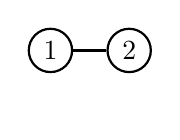
\begin{tikzpicture}[thick,
  every node/.style={circle,minimum width=.55cm, inner sep=1pt}
]
    \node[draw] (1) at (0,0) {1};
    \node[draw] (2) at (1,0) {2};
    \node[] () at (0,-.5) {};  // dummy node for padding at bottom
    \draw (1) -- (2);
\end{tikzpicture}
\qquad\quad
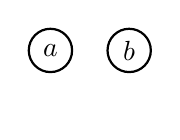
\begin{tikzpicture}[thick,
  every node/.style={circle,minimum width=.55cm, inner sep=1pt}
]
    \node[draw] (a) at (0,0) {$a$};
    \node[draw] (b) at (1,0) {$b$};
    \node[] () at (0,-.5) {};  // dummy node for padding at bottom
\end{tikzpicture}
\qquad\quad
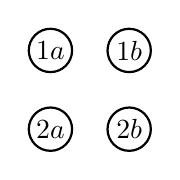
\begin{tikzpicture}[thick,
  every node/.style={draw,circle,minimum width=.55cm, inner sep=1pt}
]
    \node[draw] (1a) at (0,1) {$1a$};
    \node[draw] (1b) at (1,1) {$1b$};
    \node[draw] (2a) at (0,0) {$2a$};
    \node[draw] (2b) at (1,0) {$2b$};
\end{tikzpicture}
%%\begin{tikzpicture}[thick,
%%  every node/.style={draw,circle},
%%  class1node/.style={fill=myblue},
%%  class2node/.style={fill=mygreen},
%%  every fit/.style={ellipse,draw,inner sep=-2pt,text width=2cm}
%%]
%%        \graph [nodes={draw, circle, minimum width=.55cm, inner sep=1pt}, circular placement, radius=0.95cm,
%%                clockwise=2] {
%%                    1,2;
%%            1--2;
%%        };
%%\end{tikzpicture}
\qquad

\caption{Graphs $\graphG$ and $\graphH$ and their association graph $\graphA$.  McSplit
    gives an upper bound of 2 on the order of a maximum common induced subgraph
    of $\graphG$ and $\graphH$, whereas a clique algorithm computing
    a greedy colouring of $\graphA$ gives an tighter upper bound of 1.}
\label{fig:clique-better-bound}
\end{figure}

\Cref{fig:mcsplit-better-bound} shows an example in which McSplit's bound
may be stronger than or equal to the clique bound depending on the order in
which the greedy colouring is carried out.  The input graphs are $K_2$ and
$K_3$.  Clearly, the McSplit bound is 2.  A colouring of the association
graph has size either 2 (if we assign $1a$, $1b$, and $1c$
to one colour class, and $2a$, $2b$, and $2c$ to another) or 3 (if the
colour classes are $\{1a,2a\}$, $\{1b,2b\}$, and $\{1c,2c\}$).

\begin{figure}[h!]
\centering
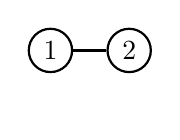
\begin{tikzpicture}[thick,
  every node/.style={circle,minimum width=.55cm, inner sep=1pt}
]
    \node[draw] (1) at (0,0) {1};
    \node[draw] (2) at (1,0) {2};
    \node[] () at (0,-.5) {};  // dummy node for padding at bottom
    \draw (1) -- (2);
\end{tikzpicture}
\qquad\quad
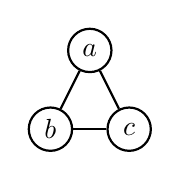
\begin{tikzpicture}[thick,
  every node/.style={circle,minimum width=.55cm, inner sep=1pt}
]
    \node[draw] (a) at (.5,1) {$a$};
    \node[draw] (b) at (0,0) {$b$};
    \node[draw] (c) at (1,0) {$c$};
    \draw (a) -- (b);
    \draw (a) -- (c);
    \draw (b) -- (c);
    %\node[] () at (0,-.5) {};  // dummy node for padding at bottom
\end{tikzpicture}
\qquad\quad
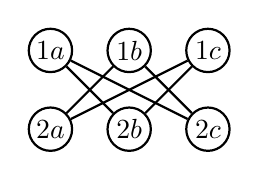
\begin{tikzpicture}[thick,
  every node/.style={draw,circle,minimum width=.55cm, inner sep=1pt}
]
    \node[draw] (1a) at (0,1) {$1a$};
    \node[draw] (1b) at (1,1) {$1b$};
    \node[draw] (1c) at (2,1) {$1c$};
    \node[draw] (2a) at (0,0) {$2a$};
    \node[draw] (2b) at (1,0) {$2b$};
    \node[draw] (2c) at (2,0) {$2c$};
    \draw (1a) -- (2b);
    \draw (1a) -- (2c);
    \draw (1b) -- (2a);
    \draw (1b) -- (2c);
    \draw (1c) -- (2a);
    \draw (1c) -- (2b);
\end{tikzpicture}
%%\begin{tikzpicture}[thick,
%%  every node/.style={draw,circle},
%%  class1node/.style={fill=myblue},
%%  class2node/.style={fill=mygreen},
%%  every fit/.style={ellipse,draw,inner sep=-2pt,text width=2cm}
%%]
%%        \graph [nodes={draw, circle, minimum width=.55cm, inner sep=1pt}, circular placement, radius=0.95cm,
%%                clockwise=2] {
%%                    1,2;
%%            1--2;
%%        };
%%\end{tikzpicture}
\qquad

\caption{Graphs $\graphG$ and $\graphH$ and their association graph $\graphA$.  McSplit
    gives an upper bound of 2 on the order of a maximum common induced subgraph
    of $\graphG$ and $\graphH$.  A greedy colouring of $\graphA$
    gives an upper bound of 2 or
    3, depending on the order in which vertices are coloured.}
\label{fig:mcsplit-better-bound}
\end{figure}

We now turn to the extreme case in which all vertex labels are distinct
in each of the two input graphs.  \Cref{fig:clique-bound-labelled} shows
two graphs, each with three distinctly-labelled vertices; the labels
are represented by three different shapes.  The McSplit upper bound is 3.
A greedy colouring of the association graph gives a stronger bound, 2,
irrespective of the order in which the nodes are coloured, since
nodes $1a$ and $3c$ will be assigned to the same colour class.

Clearly, this example generalises: if all of the vertices in each input
graph have distinct labels, then the clique bound is less than or equal to
the McSplit bound.

\begin{figure}[h!]
\centering
\begin{tikzpicture}[thick,
  triangle/.style = {regular polygon, regular polygon sides=3, inner sep=0.2pt },
  square/.style = {regular polygon, regular polygon sides=4 },
  every node/.style={circle,minimum width=.55cm, inner sep=1pt}
]
    \node[draw,triangle] (1) at (.5,1) {1};
    \node[draw,square] (2) at (0,0) {2};
    \node[draw] (3) at (1,0) {3};
    \draw (1) -- (2);
    \draw (2) -- (3);
\end{tikzpicture}
\qquad\quad
\begin{tikzpicture}[thick,
  triangle/.style = {regular polygon, regular polygon sides=3, inner sep=0.7pt },
  square/.style = {regular polygon, regular polygon sides=4 },
  every node/.style={circle,minimum width=.55cm, inner sep=1pt}
]
    \node[draw,triangle] (a) at (.5,1) {$a$};
    \node[draw,square] (b) at (0,0) {$b$};
    \node[draw] (c) at (1,0) {$c$};
    \draw (a) -- (b);
    \draw (a) -- (c);
    \draw (b) -- (c);
    %\node[] () at (0,-.5) {};  // dummy node for padding at bottom
\end{tikzpicture}
\qquad\quad
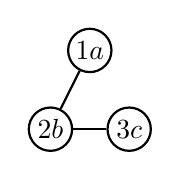
\begin{tikzpicture}[thick,
  every node/.style={draw,circle,minimum width=.55cm, inner sep=1pt}
]
    \node[draw] (1a) at (.5,1) {$1a$};
    \node[draw] (2b) at (0,0) {$2b$};
    \node[draw] (3c) at (1,0) {$3c$};
    \draw (1a) -- (2b);
    \draw (2b) -- (3c);
\end{tikzpicture}
%%\begin{tikzpicture}[thick,
%%  every node/.style={draw,circle},
%%  class1node/.style={fill=myblue},
%%  class2node/.style={fill=mygreen},
%%  every fit/.style={ellipse,draw,inner sep=-2pt,text width=2cm}
%%]
%%        \graph [nodes={draw, circle, minimum width=.55cm, inner sep=1pt}, circular placement, radius=0.95cm,
%%                clockwise=2] {
%%                    1,2;
%%            1--2;
%%        };
%%\end{tikzpicture}
\qquad

\caption{Graphs $\graphG$ and $\graphH$ and their association graph $\graphA$.
    Vertex labels are represented by shapes.  McSplit
    gives an upper bound of 3 on the order of a maximum common induced subgraph
    of $\graphG$ and $\graphH$.  A greedy colouring of $\graphA$
    gives an upper bound of 2.}
\label{fig:clique-bound-labelled}
\end{figure}

We have established that the McSplit and clique upper bounds are incomparable for unlabelled graphs,
and that the clique algorithm's bound is stronger than the McSplit bound if there are very many vertex
labels.  To find out which bound is better in practice for unlabelled graphs, and to find the point
at which the clique bound becomes preferable, I carried out a small experiment on $G(n,p)$ random graphs,
variying the size of the set of vertex labels.

I generated 1800 pairs of random undirected, loopless graphs of order 20 without edge labels,
with densities ranging from $0.1$ to $0.9$
in steps of $0.1$.  For each integer value of a parameter $m$ (the maximum label) from 1 to 20, I generated
90 pairs of graphs with vertex labels randomly assigned from the set $\{1,\dots,m\}$.  I used my
implementation of McSplit and Patrick Prosser's implementation of the MCSa1 algorithm
\cite{DBLP:journals/algorithms/Prosser12} to find the McSplit and clique bounds respectively
at the top of search (that is, on the first recursive call, before any vertex assignment decisions
have been made).

\Cref{figure:bound-ratio} plots the results of dividing the McSplit upper bound by the
clique upper bound, with one point per instance.  The value of $m$ parameter is shown on the horizontal
axis; points towards the right of the plot have more distinct vertex labels.  Mean values
are shown as horizontal lines.  When $m=1$---that is,
when all vertices have the same label---the McSplit bound is strictly tighter than the clique-algorithm
bound of all 90 of our instances.  On average, the McSplit bound is tighter than than the clique
bound for $m < 4$, and worse than the clique bound for $m > 5$.  Of the 900 instances with $m > 10$,
McSplit had a tighter bound than the clique algorithm for only a single instance.

\begin{figure}[h!]
    \centering
    \includegraphics*[width=0.65\textwidth]{14-mcsplit-i-undirected/bound-experiments/plots/bounds-plot.pdf}
    \caption{As the number of vertex labels is increased, the clique algorithm's bound
    	becomes stronger than the McSplit bound.
        The vertical axis shows the ratio of initial McSplit upper bound
	to initial clique algorithm (MCSa1) upper bound for 1800 instances, with one dot per instance;
	for values less than 1, McSplit's bound is better than that of the clique algorithm.
	The horizontal axis shows the maximum label $m$; each vertex label is a random integer 
	from the range $[1,m]$.}
    \label{figure:bound-ratio}
\end{figure}

\hrule

A further advantage of our encoding is that it gives us efficient access to a
better branching heuristic. The CP-FC algorithm uses smallest domain first,
which in our algorithm corresponds to branching on a label class with smallest
$|\setH|$. We instead branch on the label class with smallest $\max(|\setG|,|\setH|)$.
This is empirically better, and accounts for much of the difference between
the number of recursive calls made; branching on the smallest $|\setG| |\setH|$ gives
very similar results. This can be viewed as exploiting both smallest domain first,
and the dual viewpoint \citep{DBLP:conf/ecai/Geelen92} of smallest domain
first, simultaneously, but we do not have the overheads of having to maintain
and channel between the dual viewpoint that would be required when using a
conventional domain store.

What about our relationship to the $k{\downarrow}$ of
\citet{UpcomingAAAIPaper}?  \Cref{figure:prettyheatmaps3} plots the number of
recursive calls made by $k{\downarrow}$ and \McSplit{$\downarrow$} on each of the subgraph
isomorphism instances. Although \McSplit{$\downarrow$} is the faster of the two algorithms overall, it
explores more search nodes than $k{\downarrow}$ for most instances (even taking
into account that $k{\downarrow}$ uses a unit propagation loop, and so measures
the search tree slightly differently). This is the classic tradeoff between
speed and cleverness. A hybrid algorithm could be beneficial here: it could use
$k{\downarrow}$ initially, switching to \McSplit{$\downarrow$} when the extra filtering is
ineffective, and finally switching to a clique encoding when fewer than some
threshold number of vertices remain to be selected. This might deliver the
benefits of the clique encoding for labelled graphs, while avoiding the high
memory cost and colouring time of encoding the full instance.

\section{Proof of correctness}

This section proves the correctness of the variant of McSplit in \cref{DecisionMcSplitAlg}, which solves
the decision variant of maximum common induced subgraph: given two graphs and a natural number
$t$ (the ``target''), does there exist a common induced subgraph with at least $t$ vertices?
(The circled letters should be ignored for now.)
This algorithm contains all of the ingredients of the full McSplit algorithm (\cref{McSplitAlg})
other than the branch-and-bound technique; by removing branch and bound we can give a simpler
proof that focuses on the details that are specific to McSplit.  At the end of the section,
I will describe how the proof can be extended to the full branch-and-bound McSplit algorithm.

\begin{algorithm}[h!]
\DontPrintSemicolon
\nl $\FuncSty{Search}(\AlgVar{future},M,t)$ \;
\nl \Begin{
    \nl \lIf {$|M| = t$}{\KwSty{return} $\AlgVar{true}$ \algstep{A}} \label{DecisionReturnTrue}
\nl $\AlgVar{bound} \gets |M|  + \sum_{\langle \setG,\setH \rangle \in \AlgVar{future}} \min(|\setG|,|\setH|)$ \label{DecisionCalcBound} \;
\nl \lIf {$\AlgVar{bound} < t$}{\KwSty{return} $\AlgVar{false}$ \algstep{B}} \label{DecisionPruneSearch}
\medskip
\nl $\langle \setG,\setH \rangle \gets \FuncSty{SelectLabelClass}(\AlgVar{future})$ \label{DecisionSelectClass} \;
\nl $v \gets \FuncSty{SelectVertex}(\setG)$ \label{DecisionSelectVertex} \;
    \nl \For {$w \in \setH$ \algstep{C} \label{DecisionWLoop}} {
\nl    $\AlgVar{future'} \gets \emptyset$ \label{DecisionNewFuture} \;
\nl    \For {$\langle \setG',\setH'\rangle \in future$ \label{DecisionInnerLoop}}{
\nl        $\setG'' \gets \setG' \cap \N(\graphG, v) \setminus \{v\}$ \label{DecisionNewPWithEdge} \;
\nl        $\setH'' \gets \setH' \cap \N(\graphH, w) \setminus \{w\}$ \;
\nl        \If {$\setG'' \neq \emptyset$ \bf{and} $\setH'' \neq \emptyset$\label{DecisionIfNonEmpty}}{
\nl            $\AlgVar{future'} \gets \AlgVar{future'} \cup \{\langle \setG'' , \setH'' \rangle\}$ \label{DecisionAddToFutureWithEdge}}
\nl        $\setG'' \gets \setG' \cap \invN(\graphG, v) \setminus \{v\}$ \label{DecisionNewPWithoutEdge}  \;
\nl        $\setH'' \gets \setH' \cap \invN(\graphH, w) \setminus \{w\}$ \;
\nl        \If {$\setG'' \neq \emptyset$ \bf{and} $\setH'' \neq \emptyset$\label{DecisionIfNonEmpty2}}{
\nl            $\AlgVar{future'} \gets \AlgVar{future'} \cup \{\langle \setG'' , \setH'' \rangle\}$} \label{DecisionInnerLoopEnd}
       }
\nl   \lIf {$\FuncSty{Search}(\AlgVar{future'},M\cup \{(v,w)\},t)$ \label{DecisionExpandWithV}}{$\KwSty{return}$ $\AlgVar{true}$ \algstep{D}}
  }
\nl $\setG' \gets \setG \setminus \{v\}$ \label{DecisionRemoveV} \;
\nl $\AlgVar{future'} \gets \AlgVar{future} \setminus \{\langle \setG,\setH \rangle\}$\;
\nl \lIf {$\setG' \neq \emptyset$} {$\AlgVar{future'} \gets \AlgVar{future'} \cup \{\langle \setG',\setH \rangle \}$}
\nl \lIf {$\FuncSty{Search}(\AlgVar{future'},M,t)$ \label{DecisionExpandWithoutV}}{$\KwSty{return}$ $\AlgVar{true}$ \algstep{E}}
    \nl  $\KwSty{return}$ $\AlgVar{false}$ \algstep{F}\;
}
\;
\nl $\FuncSty{McSplitDecision}(\graphG,\graphH, t)$ \label{DecisionMcSplitFun} \;
\nl \Begin{
\nl $\KwSty{return}$ $\FuncSty{Search}(\{\langle V(\graphG),V(\graphH) \rangle \},\emptyset, t)$ \label{DecisionFirstExpandCall} \;
}
\caption{A decision-problem variant of McSplit.}
\label{DecisionMcSplitAlg}
\end{algorithm}

For simplicity, we will assume that the input graphs are unlabelled,
undirected and loopless.
Our proof uses the well-known fact that a common subgraph with $t$ vertices exists
if and only if the association graph (also known as the weak modular product graph)
has a clique with $t$ vertices \cite{LeviG}.  The association graph of $\graphG$ 
$\graphH$, which we will
call $\graphA$, is defined as follow.  The vertex set of $\graphA$ is
$V(\graphG) \times V(\graphH)$.  Two vertices $(v,w)$ and $(v',w')$ of $\graphA$
are adjacent if and only if $v \not= v'$, $w \not= w'$, and either (1) $v$ and $v'$
are adjacent in $\graphG$ and $w$ and $w'$ are adjacent in $\graphH$ or (2) $v$ and $v'$
are not adjacent in $\graphG$ and $w$ and $w'$ are not adjacent in $\graphH$.

\Cref{fig:association-graph} shows the association graph of graphs $\graphG$ and $\graphH$
from \cref{fig:alg1}, which has 30 vertices and 150 edges.  A 4-clique corresponding to
a maximum common subgraph of $\graphG$ and $\graphH$ is shown.

\begin{figure}[htb]
\centering
    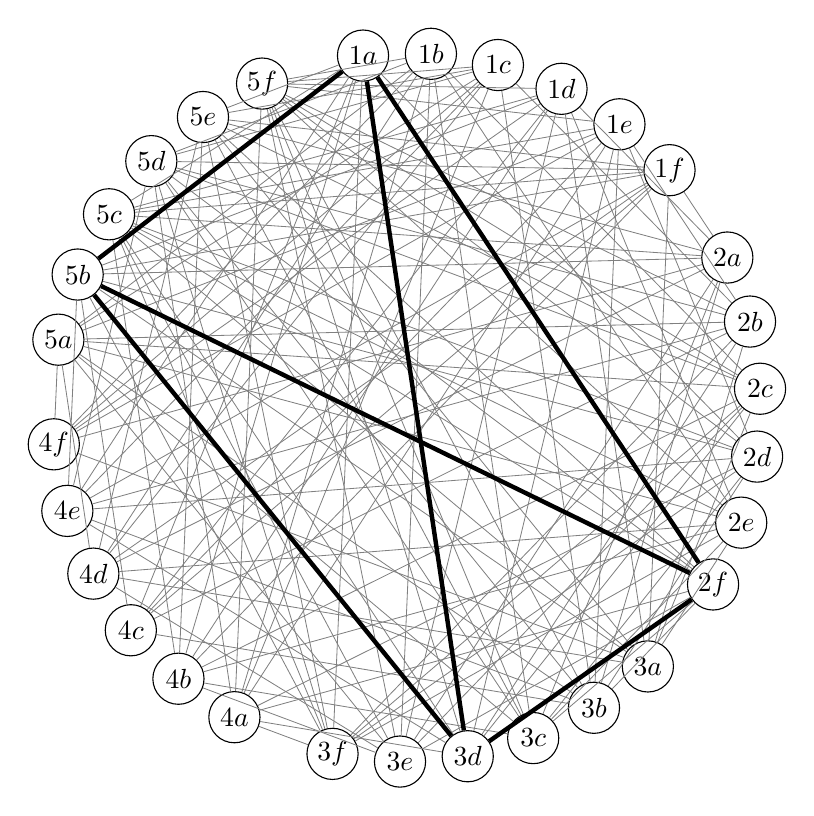
\begin{tikzpicture}
        \foreach \v [count=\i] in {1,2,3,4,5} {
            \foreach \w [count=\j] in {a,b,c,d,e,f} {
                \node[draw,circle,minimum width=.65cm,inner sep=1pt] (\v\w) at (180 - \i*72 - \j*11:4.5) {$\v\w$};
            }
        }
        \draw[color=gray, line width=.3] (1a) -- (2d);
\draw[color=gray, line width=.3] (1a) -- (3f);
\draw[color=gray, line width=.3] (1a) -- (4b);
\draw[color=gray, line width=.3] (1a) -- (4c);
\draw[color=gray, line width=.3] (1a) -- (4e);
\draw[color=gray, line width=.3] (1a) -- (5c);
\draw[color=gray, line width=.3] (1a) -- (5e);
\draw[color=gray, line width=.3] (1b) -- (2c);
\draw[color=gray, line width=.3] (1b) -- (2e);
\draw[color=gray, line width=.3] (1b) -- (3c);
\draw[color=gray, line width=.3] (1b) -- (3e);
\draw[color=gray, line width=.3] (1b) -- (4a);
\draw[color=gray, line width=.3] (1b) -- (4d);
\draw[color=gray, line width=.3] (1b) -- (4f);
\draw[color=gray, line width=.3] (1b) -- (5a);
\draw[color=gray, line width=.3] (1b) -- (5d);
\draw[color=gray, line width=.3] (1b) -- (5f);
\draw[color=gray, line width=.3] (1c) -- (2b);
\draw[color=gray, line width=.3] (1c) -- (3b);
\draw[color=gray, line width=.3] (1c) -- (4a);
\draw[color=gray, line width=.3] (1c) -- (4d);
\draw[color=gray, line width=.3] (1c) -- (4e);
\draw[color=gray, line width=.3] (1c) -- (4f);
\draw[color=gray, line width=.3] (1c) -- (5a);
\draw[color=gray, line width=.3] (1c) -- (5d);
\draw[color=gray, line width=.3] (1c) -- (5e);
\draw[color=gray, line width=.3] (1c) -- (5f);
\draw[color=gray, line width=.3] (1d) -- (2a);
\draw[color=gray, line width=.3] (1d) -- (2e);
\draw[color=gray, line width=.3] (1d) -- (3a);
\draw[color=gray, line width=.3] (1d) -- (3e);
\draw[color=gray, line width=.3] (1d) -- (4b);
\draw[color=gray, line width=.3] (1d) -- (4c);
\draw[color=gray, line width=.3] (1d) -- (4f);
\draw[color=gray, line width=.3] (1d) -- (5b);
\draw[color=gray, line width=.3] (1d) -- (5c);
\draw[color=gray, line width=.3] (1d) -- (5f);
\draw[color=gray, line width=.3] (1e) -- (2b);
\draw[color=gray, line width=.3] (1e) -- (2d);
\draw[color=gray, line width=.3] (1e) -- (3b);
\draw[color=gray, line width=.3] (1e) -- (3d);
\draw[color=gray, line width=.3] (1e) -- (4a);
\draw[color=gray, line width=.3] (1e) -- (4c);
\draw[color=gray, line width=.3] (1e) -- (4f);
\draw[color=gray, line width=.3] (1e) -- (5a);
\draw[color=gray, line width=.3] (1e) -- (5c);
\draw[color=gray, line width=.3] (1e) -- (5f);
\draw[color=gray, line width=.3] (1f) -- (2a);
\draw[color=gray, line width=.3] (1f) -- (3a);
\draw[color=gray, line width=.3] (1f) -- (4b);
\draw[color=gray, line width=.3] (1f) -- (4c);
\draw[color=gray, line width=.3] (1f) -- (4d);
\draw[color=gray, line width=.3] (1f) -- (4e);
\draw[color=gray, line width=.3] (1f) -- (5b);
\draw[color=gray, line width=.3] (1f) -- (5c);
\draw[color=gray, line width=.3] (1f) -- (5d);
\draw[color=gray, line width=.3] (1f) -- (5e);
\draw[color=gray, line width=.3] (2a) -- (3b);
\draw[color=gray, line width=.3] (2a) -- (3c);
\draw[color=gray, line width=.3] (2a) -- (3e);
\draw[color=gray, line width=.3] (2a) -- (4d);
\draw[color=gray, line width=.3] (2a) -- (4f);
\draw[color=gray, line width=.3] (2a) -- (5b);
\draw[color=gray, line width=.3] (2a) -- (5c);
\draw[color=gray, line width=.3] (2a) -- (5e);
\draw[color=gray, line width=.3] (2b) -- (3a);
\draw[color=gray, line width=.3] (2b) -- (3d);
\draw[color=gray, line width=.3] (2b) -- (3f);
\draw[color=gray, line width=.3] (2b) -- (4c);
\draw[color=gray, line width=.3] (2b) -- (4e);
\draw[color=gray, line width=.3] (2b) -- (5a);
\draw[color=gray, line width=.3] (2b) -- (5d);
\draw[color=gray, line width=.3] (2b) -- (5f);
\draw[color=gray, line width=.3] (2c) -- (3a);
\draw[color=gray, line width=.3] (2c) -- (3d);
\draw[color=gray, line width=.3] (2c) -- (3e);
\draw[color=gray, line width=.3] (2c) -- (3f);
\draw[color=gray, line width=.3] (2c) -- (4b);
\draw[color=gray, line width=.3] (2c) -- (5a);
\draw[color=gray, line width=.3] (2c) -- (5d);
\draw[color=gray, line width=.3] (2c) -- (5e);
\draw[color=gray, line width=.3] (2c) -- (5f);
\draw[color=gray, line width=.3] (2d) -- (3b);
\draw[color=gray, line width=.3] (2d) -- (3c);
\draw[color=gray, line width=.3] (2d) -- (3f);
\draw[color=gray, line width=.3] (2d) -- (4a);
\draw[color=gray, line width=.3] (2d) -- (4e);
\draw[color=gray, line width=.3] (2d) -- (5b);
\draw[color=gray, line width=.3] (2d) -- (5c);
\draw[color=gray, line width=.3] (2d) -- (5f);
\draw[color=gray, line width=.3] (2e) -- (3a);
\draw[color=gray, line width=.3] (2e) -- (3c);
\draw[color=gray, line width=.3] (2e) -- (3f);
\draw[color=gray, line width=.3] (2e) -- (4b);
\draw[color=gray, line width=.3] (2e) -- (4d);
\draw[color=gray, line width=.3] (2e) -- (5a);
\draw[color=gray, line width=.3] (2e) -- (5c);
\draw[color=gray, line width=.3] (2e) -- (5f);
\draw[color=gray, line width=.3] (2f) -- (3b);
\draw[color=gray, line width=.3] (2f) -- (3c);
\draw[color=gray, line width=.3] (2f) -- (3e);
\draw[color=gray, line width=.3] (2f) -- (4a);
\draw[color=gray, line width=.3] (2f) -- (5c);
\draw[color=gray, line width=.3] (2f) -- (5d);
\draw[color=gray, line width=.3] (2f) -- (5e);
\draw[color=gray, line width=.3] (3a) -- (4d);
\draw[color=gray, line width=.3] (3a) -- (4f);
\draw[color=gray, line width=.3] (3a) -- (5b);
\draw[color=gray, line width=.3] (3a) -- (5c);
\draw[color=gray, line width=.3] (3a) -- (5e);
\draw[color=gray, line width=.3] (3b) -- (4c);
\draw[color=gray, line width=.3] (3b) -- (4e);
\draw[color=gray, line width=.3] (3b) -- (5a);
\draw[color=gray, line width=.3] (3b) -- (5d);
\draw[color=gray, line width=.3] (3b) -- (5f);
\draw[color=gray, line width=.3] (3c) -- (4b);
\draw[color=gray, line width=.3] (3c) -- (5a);
\draw[color=gray, line width=.3] (3c) -- (5d);
\draw[color=gray, line width=.3] (3c) -- (5e);
\draw[color=gray, line width=.3] (3c) -- (5f);
\draw[color=gray, line width=.3] (3d) -- (4a);
\draw[color=gray, line width=.3] (3d) -- (4e);
\draw[color=gray, line width=.3] (3d) -- (5c);
\draw[color=gray, line width=.3] (3d) -- (5f);
\draw[color=gray, line width=.3] (3e) -- (4b);
\draw[color=gray, line width=.3] (3e) -- (4d);
\draw[color=gray, line width=.3] (3e) -- (5a);
\draw[color=gray, line width=.3] (3e) -- (5c);
\draw[color=gray, line width=.3] (3e) -- (5f);
\draw[color=gray, line width=.3] (3f) -- (4a);
\draw[color=gray, line width=.3] (3f) -- (5b);
\draw[color=gray, line width=.3] (3f) -- (5c);
\draw[color=gray, line width=.3] (3f) -- (5d);
\draw[color=gray, line width=.3] (3f) -- (5e);
\draw[color=gray, line width=.3] (4a) -- (5d);
\draw[color=gray, line width=.3] (4a) -- (5f);
\draw[color=gray, line width=.3] (4b) -- (5c);
\draw[color=gray, line width=.3] (4b) -- (5e);
\draw[color=gray, line width=.3] (4c) -- (5b);
\draw[color=gray, line width=.3] (4d) -- (5a);
\draw[color=gray, line width=.3] (4d) -- (5e);
\draw[color=gray, line width=.3] (4e) -- (5b);
\draw[color=gray, line width=.3] (4e) -- (5d);
\draw[color=gray, line width=.3] (4f) -- (5a);
\draw[ultra thick] (1a) -- (2f);
\draw[ultra thick] (1a) -- (3d);
\draw[ultra thick] (1a) -- (5b);
\draw[ultra thick] (2f) -- (3d);
\draw[ultra thick] (2f) -- (5b);
\draw[ultra thick] (3d) -- (5b);

    \end{tikzpicture}   
\caption{The association graph of graphs $\graphG$ and $\graphH$ from \cref{fig:alg1}.  The dark edges
    show a 4-clique in
    the association graph. This corresponds to a common subgraph with 4 vertices: the subgraph of $\graphG$ induced by
    $\{1,2,3,5\}$ which is isomorphic to the subgraph of $\graphH$ induced by $\{a,f,d,b\}$.}
\label{fig:association-graph}
\end{figure}

\paragraph{An algorithm for the clique decision problem}
Our proof strategy is to introduce and prove a simple algorithm for the clique
decision problem, and then to show that this algorithm, when applied to the association
graph, carries out exactly the same steps as the McSplit algorithm applied to graphs
$\graphG$ and $\graphH$.  The clique algorithm we will use, \cref{CliqueDecisionAlg},
uses a similar upper-bounding strategy to MCSa1 \cite{DBLP:journals/algorithms/Prosser12,DBLP:journals/ieicet/TomitaSHW13};
both algorithms greedily colour the vertices of the graph and use the number of colours
as an upper bound on the number of vertices that can be added to the growing clique.
\Cref{CliqueDecisionAlg} does not specify the order in which vertices are coloured;
our proof will require the colouring to mimic McSplit's behaviour, and I will give
more details on this below.

\begin{algorithm}[h!]
\DontPrintSemicolon
\nl $\FuncSty{CliqueSearch}(P,C,t)$ \;
\nl \KwData{Candidate vertices $P$, clique $C$ such that $|C| \leq t$, and target size $t$}
\nl \KwResult{$\AlgVar{true}$ if and only if a clique of size $t$ exists with $C$ as a subset}
\nl \Begin{
\nl \lIf {$|C| = t$}{\KwSty{return} $\AlgVar{true}$ \algstep{A}} \label{CliqueReturnTrue}
\nl $\AlgVar{bound} \gets |C|  + \FuncSty{ColouringUpperBound}(P)$ \label{CliqueCalcBound} \;
\nl \lIf {$\AlgVar{bound} < t$}{\KwSty{return} $\AlgVar{false}$ \algstep{B}} \label{CliquePruneSearch}
\medskip
\nl $S \gets $ a subset of $P$ that is an independent set in $\graphA$ \label{CliqueChooseS} \;
    \nl \For {$x \in S$ \algstep{C}\label{CliqueWLoop}} {
    \nl    \lIf {$\FuncSty{CliqueSearch}(P \cap N(x), C \cup \{x\}, t)$}{\KwSty{return} $\AlgVar{true}$ \algstep{D}\label{CliqueFirstSearch}}
     }
    \nl  \lIf {$\FuncSty{CliqueSearch}(P \setminus S, C, t)$}{\KwSty{return} $\AlgVar{true}$ \algstep{E}\label{CliqueSecondSearch}}
  \nl  $\KwSty{return}$ $\AlgVar{false}$ \algstep{F}\;
  }
\;
\nl $\FuncSty{ColouringUpperBound}(P)$ \;
\nl \KwData{Candidate vertices $P$}
\nl \KwResult{An upper bound on the size of a clique containing only vertices in $P$}
\nl \Begin{
\nl   Greedily colour the subgraph of $\graphA$ induced by $P$, and return the size of this colouring.
  }
\;
\nl $\FuncSty{Clique}(\graphA, t)$ \label{CliqueFun} \;
\nl \KwData{Graph $\graphA$ and target size $t$}
\nl \KwResult{$\AlgVar{true}$ if and only if a clique of size $t$ exists in $\graphA$}
\nl \Begin{
\nl $\KwSty{return}$ $\FuncSty{CliqueSearch}(V(\graphA),\emptyset, t)$ \label{CliqueFirstExpandCall} \;
}
\caption{A simple algorithm for the clique decision problem.}
\label{CliqueDecisionAlg}
\end{algorithm}

Our clique algorithm uses a simpler branching strategy than MCSa1.

The parameters of the $\FuncSty{CliqueSearch}$ function of \cref{CliqueDecisionAlg}
are vertex sets $P$ and $C$ and a natural number $t$.  Set $C$ is a subset of
$V(\graphA)$, and must be a clique of size no greater than $t$. Set $P$ is a
set of candidate (``potential'') vertices, sucht that $C \cap P = \emptyset$
and each vertex in $P$ is adjacent in $\graphA$ to every member of $C$.  The
parameter $t$ is the target clique size.  We now show the correctness of the
algorithm.

\begin{proposition}\label{cliqueAlgProp}
    The function $\FuncSty{CliqueSearch}(P,C,t)$ returns $\AlgVar{true}$ if and only if $\graphA$ has a clique
  $K$ of size $t$ such that $C \subseteq K \subseteq C \cup P$.
\end{proposition}
\begin{proof}
  The proof is by induction on $|P|$.
  
  \emph{Base case, $|P|=0$.} Since $C$ is a clique by assumption and $P = \emptyset$,
    we must show that the function returns $\AlgVar{true}$ if and only if $|C| = t$.
    If $|C| = t$, \lineref{CliqueReturnTrue} returns $\AlgVar{true}$ as required.
    If $|C| < t$, then $\AlgVar{bound} = |C|$, since $\FuncSty{ColouringUpperBound}(P)$
    is zero. Therefore $\AlgVar{false}$ is returned on \lineref{CliquePruneSearch}.

  \emph{Inductive case.} Let natural number $k$ be given, and assume that the proposition holds
    for $|P| < k$. We will show that the proposition also holds if $|P| = k$.  Let $C$, $P$,
    and $t$ be given, such that $|P| = k$.

  For the first direction of the implication in the inductive case, suppose there is no clique
  $K$ of size $t$ such that $C \subseteq K \subseteq C \cup P$.  \Lineref{CliqueReturnTrue}
  does not return $\boolT$ since $|C| < t$. Now, either \cref{CliquePruneSearch} returns \boolF\
  or we must show that neither \lineref{CliqueFirstSearch} nor \lineref{CliqueSecondSearch}
  returns \boolT. We first consider \lineref{CliqueFirstSearch}. By assumption, for every clique $K$
  of size $t$ we have either that $C \not\subseteq K$ or $K \not\subseteq C \cup P$.  Since
  $C \subset C \cup \{x\}$ and $C \cup \{x\} \cup (P \cap N(x)) \subseteq C \cup P$, it follows
  for every clique $K$ of size $t$ that either
  $C \cup \{x\} \not\subseteq K$ or $K \not\subseteq C \cup \{x\} \cup (P \cap N(x))$.  Hence
  the call to $\FuncSty{CliqueSearch}()$ on \lineref{CliqueFirstSearch} returns \boolF
  for every value taken by $x$ in the loop.  It remains to show
  that \lineref{CliqueSecondSearch}, if reached, never returns \boolT; this is the case since
  $P \setminus S \subset P$ and therefore for every clique $K$ of size $t$ we have either
  $C \not\subseteq K$ or $K \not\subseteq C \cup (P \setminus S)$.

  For the second direction of the implication in the inductive case, suppose there exists a clique
  $K$ of size $t$ such that $C \subseteq K \subseteq C \cup P$.  If $|C|=t$, \Lineref{CliqueReturnTrue}
  returns \boolT\ as required.  Otherwise, $\AlgVar{bound} \geq t$ since $K \setminus C$ is a clique
  and therefore each member of $K \setminus C$ must be in a different colour class in the colouring
    generated by the function $\FuncSty{ColouringUpperBound}$; therefore, \lineref{CliquePruneSearch}
    does not return \boolF.  It remains to show that either 
  \lineref{CliqueFirstSearch} or \lineref{CliqueSecondSearch} returns \boolT. We consider two
  cases: $S \cap K \not= \emptyset$ and $S \cap K = \emptyset$.  In the first case, let $x$ be
  the unique element of $S \cap K$.  Since $C \subseteq K$ and $x \in K$, we have
  $C \cup \{x\} \subseteq K$.
  Since $K$ is a clique containing $x$, we have $K \subseteq \{x\} \cup N(x)$ and
    therefore $P \cap K \subseteq \{x\} \cup (P \cap N(x))$.
  Combining this with the fact that $K \subseteq C \cup P$,
  we have $K \subseteq C \cup \{x\} \cup (P \cap N(x))$.  It follows directly that \lineref{CliqueFirstSearch}
  returns \boolT.

    Now consider the second case: $S \cap K = \emptyset$.  Since $K \subseteq C \cup P$,
    we have $K \subseteq C \cup (P \setminus S)$.  Therefore \lineref{CliqueSecondSearch}
    returns \boolT.
\end{proof}

\paragraph{Equivalence of \cref{DecisionMcSplitAlg} and \cref{CliqueDecisionAlg}.}  We will now show
that \cref{DecisionMcSplitAlg} and \cref{CliqueDecisionAlg} explore the same search tree.
Suppose we have graphs $\graphG$ and $\graphH$ for which we wish to find a common subgraph,
and their association graph $\graphA$.
We will consider calls to $\FuncSty{Search}(\AlgVar{future},M,t)$ in the McSplit algorithm,
and corresponding calls $\FuncSty{CliqueSearch}(P,C,t)$ in the clique algorithm, where
$P = \{G \times H \mid \langle G,H \rangle \in \AlgVar{future}\}$ and $C = M$.  That is,
each call to the $\FuncSty{CliqueSearch}()$ function takes as its $P$ argument a set containing
every node $(v,w)$ in the association graph such that $v$ and $w$ are in the same label class 
in $\AlgVar{future}$, and as its $C$ argument every node $(v,w)$ in the association graph corresponding
to an assignment in $M$.

In order for the two algorithms
to explore equivalent search trees, we must make precise
the $\FuncSty{ColouringUpperBound}()$ function and the procedure for selecting independent set $S$ on
\lineref{CliqueChooseS} of \cref{CliqueDecisionAlg}.  The $\FuncSty{ColouringUpperBound}(P)$ call
returns the size of a colouring of $P = \{G \times H \mid \langle G,H \rangle \in \AlgVar{future}\}$
in the association graph.  For each $\langle G, H\rangle$ in $\AlgVar{future}$, we colour the corresponding
subset of $P$, that is, $G \times H$, as follows.  If $|G| \leq |H|$, we assign a colour to the set
of association graph nodes $\{(v,w) \mid w \in H\}$ for each $v \in G$.  If $|G| > |H|$, we assign
a colour to the set of association graph nodes $\{(v,w) \mid v \in G\}$ for each $w \in H$.
The subset of $P$ corresponding to label class $\langle G,H \rangle$ therefore requires
$\min(|\setG|,|\setH|)$ colours.
The size of the colouring returned by $\FuncSty{ColouringUpperBound}(P)$ is
$\sum_{\langle \setG,\setH \rangle \in \AlgVar{future}} \min(|\setG|,|\setH|)$.

We now turn to \lineref{CliqueChooseS} of \cref{CliqueDecisionAlg}, which chooses an independent
set of nodes from $P$ on which to branch.  We choose $S = \{(v,w) \mid w \in H\}$, with $H$
and $v$ taking the values selected by $\FuncSty{SelectLabelClass}(\AlgVar{future})$
and $\FuncSty{SelectVertex}(G)$ on lines \lineref{DecisionSelectClass} and \lineref{DecisionSelectVertex}
of \cref{DecisionMcSplitAlg}.  This ensures that the branching decisions in the clique algorithm
mirror those of the McSplit algorithm.

\begin{proposition}\label{cliqueMcSplitProp}
    Let graphs $\graphG$ and $\graphH$ be given, and let $\graphA$ be their association graph.
    Let a set of label classes $\AlgVar{future}$, a mapping $M$, and a target size $t$ be given.
    Let $P$ be the set of association-graph nodes corresponding to $\AlgVar{future}$; that is,
    $P = \{G \times H \mid \langle G,H \rangle \in \AlgVar{future}\}$.  Let $C = M$.
    The function $\FuncSty{CliqueSearch}(P,C,t)$ returns the same value as
    $\FuncSty{Search}(\AlgVar{future},M,t)$.
\end{proposition}
\begin{proof}
  The proof is by induction on $|P|$.

  \emph{Base case, $|P|=0$.} If $|M| = t$, both algorithms return \boolT\ at
    the line marked \algstep{A}.  Otherwise, $\AlgVar{bound} = |M|$ and both
    algorithms return \boolF\ at the line marked \algstep{B}.

  \emph{Inductive case.} Both algorithms return \boolT\ at the line marked
    \algstep{A} if and only if $|M|=t$.  We have shown that $\FuncSty{ColouringUpperBound}(P) =
    \sum_{\langle \setG,\setH \rangle \in \AlgVar{future}} \min(|\setG|,|\setH|)$; therefore,
    both algorithms return \boolF\ at the line marked \algstep{B} if and only
    if 
\[
    |M| + \sum_{\langle \setG,\setH \rangle \in \AlgVar{future}} \min(|\setG|,|\setH|) < t.
\]
    Due to the way we have defined set $S$, the loop marked \algstep{C} in the clique
    algorithm iterates over the set $\{(v,w) \mid w \in H\}$, where $H$ is the set
    iterated over in the corresponding loop of the McSplit algorithm.  To show that the lines
    marked \algstep{D} are equivalent in the two algorithms, we must show that
    $P \cap N(\graphA, (v,w)) = \{G \times H \mid \langle G,H \rangle \in \AlgVar{future'}\}$
    (where $(v,w)$ is the value of loop variable $x$ in the clique algorithm), and that
    $C \cup \{(v,w)\} = M \cup \{(v,w)\}$.  The latter equality is trivial.

    To prove one direction of inclusion in the former equality, let $(v',w')$
    be an element of $P \cap N(\graphA, (v,w))$.  Since, by definition, $P =
    \{G \times H \mid \langle G,H \rangle \in \AlgVar{future}\}$, there exists
    a label class $\langle G',H' \rangle \in \AlgVar{future}$ such that $v \in
    G'$ and $w \in H'$.  Since $(v',w') \in N(\graphA, (v,w))$, we have that $v
    \not= v'$, $w \not= w'$, and either (1) $v$ and $v'$ are adjacent and $w$
    and $w'$ are adjacent or (2) $v$ and $v'$ are non-adjacent and $w$ and $w'$
    are non-adjacent.  In the first of these cases, a label class containing
    $v'$ and $w'$ will be added to $\AlgVar{future'}$ on
    \lineref{DecisionAddToFutureWithEdge}.  In the second case, a label class
    containing $v'$ and $w'$ will be added to $\AlgVar{future'}$ on
    \lineref{DecisionInnerLoopEnd}. In either case, $(v',w')$ will be an
    element of $\{G \times H \mid \langle G,H \rangle \in \AlgVar{future'}\}$,
    as required.

    To prove the second direction of inclusion, let $v'$ and $w'$ be such that for
    some element $\langle G'',H'' \rangle$ of $\AlgVar{future'}$, we have
    $v' \in G''$ and $w' \in H''$.  It must hold that 
    $\langle G'',H'' \rangle$ was added to $\AlgVar{future'}$ either on
    \lineref{DecisionAddToFutureWithEdge} or \lineref{DecisionInnerLoopEnd} of
    \cref{DecisionMcSplitAlg}. In the former case, by the construction of $G''$ and $H''$
    in \cref{DecisionMcSplitAlg}, we have that $v$ and $v'$ are distinct and adjacent
    in $\graphG$ and that $w$ are $w'$ are distinct and adjacent in $\graphH$.
    Therefore, $(v',w')$ is an element
    of $N(\graphA, (v,w))$.
    Moreover, again by the construction of $G''$ and $H''$,
    there is some $\langle G',H' \rangle \in \AlgVar{future}$ such that
    $v' \in G'$ and $w' \in H'$.
    Therefore, $(v',w')$ is an element of $P$.
    Thus, $(v',w')$ is an element of $P \cap N(\graphA, (v,w))$ as required.
    A similar proof applies in the case where
    $\langle G'',H'' \rangle$ was added to $\AlgVar{future'}$ on
    \lineref{DecisionInnerLoopEnd} of \cref{DecisionMcSplitAlg}.

    We now move to the lines marked \algstep{E} of the two algorithms. 
    To prove the equivalence of the two recursive calls, we must show that
    $P \setminus S = \{G \times H \mid \langle G,H \rangle \in \AlgVar{future'}\}$. We have
\begin{gather}
    P \setminus S = \\
    \{(u,w) \in \{G \times H \mid \langle G,H \rangle \in \AlgVar{future}\} \mid u \not= v\} = \\
    \{\{u \in G \mid u \not= v\} \times H \mid \langle G,H \rangle \in \AlgVar{future}\} = \\
    \{G \times H \mid \langle G,H \rangle \in \AlgVar{future'}\}.
\end{gather}

    Finally, both function return \boolF\ upon reaching the line marked \algstep{F}.
\end{proof}

It is clear from the proof of \cref{cliqueMcSplitProp} that \cref{DecisionMcSplitAlg}
and \cref{CliqueDecisionAlg} explore identically-shaped search trees.

TODO: check you've said enough about the clique bound vs McSplit bound. Possibly
re-order this in the chapter.

\paragraph{Branch and bound algorithms}
In order to simplify the exposition, this section has shown that a
decision-problem variant of McSplit is equivalent to an algorithm
for the clique decision problem.  It would be straightforward to convert our clique
algorithm into a branch and bound algorithm by introducing a global $\AlgVar{incumbent}$
variable in the style of \cref{McSplitAlg}.  The proof of \cref{cliqueMcSplitProp} could
then be modified trivially to show the equivalence of the full McSplit algorithm to
a branch-and-bound algorithm for the maximum clique problem.

\paragraph{Extensions of McSplit}
The definition of the association graph can easily be modified to handle loops,
directed edges, and labelled vertices and edges \cite{LeviG}.  It would be
possible to modify our correctness proof of McSplit to apply to any of these
variants of the problem by using an appropriate definition of the association
graph.

To solve the maximum common \emph{connected} subgraph problem with a clique algorithm,
we must distinguish between two types of edges in the association graph: $c$-edges
corresponding to edges in graphs $\graphG$ and $\graphH$, and $d$-edges corresponding
to non-edges in the two graphs.  We then search for a clique in the association graph
that is spanned by $c$-edges.
\cite{DBLP:journals/tcs/Koch01,DBLP:conf/mco/VismaraV08,DBLP:conf/cp/McCreeshNPS16}
\cite{DBLP:conf/cp/McCreeshNPS16} introduces a modified maximum-clique algorithm
that solves this problem by only choosing to add those vertices to the clique $C$ that
have at least one $c$-edge to a vertex that is already in the clique.  (The first
vertex added to $C$ is a special case and is not subject to this restriction.)
It would be straightforward to modify our clique algorithm to solve this version of the
problem, and we could then modify the proof of \cref{cliqueMcSplitProp} to prove the
correctness of the connected version of McSplit.


TODO note that this discussion shows similarity between McSplit and clique encoding

\section{Publications using McSplit}

Since the McSplit algorithm was published at IJCAI 2017, a number of papers (including
{\color{blue} TODO insert number} that I co-authored have further investigated the algorithm.
This section briefly surveys this work.

In his undergraduate thesis \cite{dilkas2018}, Paulius Dilkas performs a detailed experimental evaluation
of McSplit and a clique algorithm for a range of labelling schemes, finding that McSplit
outperforms the clique encoding even for labelled graphs, if only a small number of labels are
used.  Dilkas uses machine learning to construct a portfolio solver that chooses intelligently
between McSplit and the clique encoding according to easily-computed characteristics of the
two input graphs such as density and standard deviation of degrees. The portfolio solver
outperforms each of its component algorithms, giving overall performance close to that of the virtual
best solver.  Finally, Dilkas constructs hybrid algorithm, \textsc{Fusion}, that switches
from McSplit to the clique encoding at a specified depth of recursion.

Liu et al. \cite{DBLP:conf/aaai/0001LJ020} use reinforcement learning to create a better branching
heuristic.  Specifically, when selecting a vertex in $\graphG$ or $\graphH$ to use for branching,
the algorithm prefers to use vertices that have resulted in a large decrease to the upper bound
in previous recursive calls.  This strategy increased the speed of McSplit on maximum common subgraph
instances by around a factor of 2.  It caused an even more dramatic improvement when McSplit was
applied to the induced subgraph isomorphism problem, outperforming a leading specialised subgraph
isomorphism solver.

Archibald et al. \cite{DBLP:conf/cpaior/ArchibaldDHMP019} introduce \emph{solution-biased search},
a technique using restarts and nogood learning that allows algorithm to quickly explore diverse
parts of the search tree rather than explore it in order (as a typical backtracking algorithm
such as the standard version of McSplit does); this can often help the algorithm to find good
solutions quickly.  For the paper, I designed and implemented a version
of McSplit using solution-biased search; this led to modestly improved run times on many instances.

\section{Isolde}

TODO

\section{Some data related to Diaconis and Sourav's paper?}

TODO

\section{Conclusion}

We have introduced the \McSplit\ algorithm for maximum common subgraph
problems.  This algorithm is more than an order of magnitude faster than the
previous state of the art for unlabelled and undirected instances. We have
shown how the algorithm can be extended for graphs with labels on edges, labels
on vertices, loops, directed edges and the requirement that the resultant graph
be connected.

We believe there is more to be discovered about branching heuristics. There is
also the potential to branch on both sides, that is instead of branching on
vertices in $\V(\graphG)$, it would be equally valid to branch on a vertex in
$\V(\graphH)$, since our data structure treats the two graphs symmetrically. More
interestingly, we could choose which graph to branch on at each search node
using some heuristic (perhaps choosing based on whether the $\setG$ or $\setH$ set is
smaller).

It would be interesting to see whether these techniques are more broadly
applicable---we suspect that some other problems may have a similar branching
structure which would also benefit from a partitioning domain store
representation. Most obviously, we could solve the induced subgraph isomorphism
problem in the same way (and with nearly no changes to the code), and our
connected variant shows that certain side constraints can also be handled.
However, we cannot solve non-induced subgraph isomorphism this way, nor can
we handle certain richer labelling schemes such as those used in temporal
subgraph isomorphism \citep{DBLP:conf/asunam/RedmondC13}.
